\documentclass[a4paper, toc=index, 12pt, DIV14, twoside, BCOR2cm, headsepline, numbers=noenddot, bibliography=totoc]{report}

\usepackage{graphicx}
\usepackage{alltt}
\usepackage{url}
\usepackage{tabularx}
%\usepackage{ngerman}
\usepackage{longtable}
\usepackage[utf8]{inputenc}
\usepackage{tabularx}
\usepackage{listings}             % Include the listings-package
\usepackage{color}
\usepackage{graphicx}
\usepackage{caption}
\usepackage{subcaption}

\usepackage[T1]{fontenc}
\usepackage{ae, aecompl}
\usepackage{a4wide}
\usepackage{boxedminipage}
\usepackage{url}
\usepackage{graphicx}
\usepackage{enumerate}
\usepackage{float}
\usepackage{multicol}
\usepackage{tabularx}


\usepackage{ifthen}
\raggedbottom

\newenvironment{prettytablex}[1]{\vspace{0.3cm}\noindent\tabularx{\linewidth}{@{\hspace{\parindent}}#1@{}}}{\endtabularx\vspace{0.3cm}}
\newenvironment{prettytable}{\prettytablex{l X}}{\endprettytablex}
\setcounter{secnumdepth}{3}
\setcounter{tocdepth}{3}


\title{\huge\sffamily\bfseries System Description and Risk Analysis}
\author{Marc G\"ahwiler \and Leonhard Helminger \and Fabian Zeindler}
\date{21.11.2013}


\begin{document}
\maketitle

\tableofcontents
\pagebreak


\chapter{System Characterization}
\section{Introduction}
The company iMovies produces film material in the area of investigative journalism. To protect the integrity and the secrecy of email conversations within the company, a certificate based solution should be provided which ensures the confidentiality of these email conversations.\newline
Today the IT infrastructure of the company is divided into an internal network where the employees work with their desktop machines/laptops and a server area in which the a database server with user data, the web and email server as well as central storage for the employees are located. (this is an assumption by us, since there is no information about the status quo and iMovies is a relatively small company.) The status quo of the system is depicted in Figure \ref{oldsystem}.

\begin{figure}[H]
  \centering
    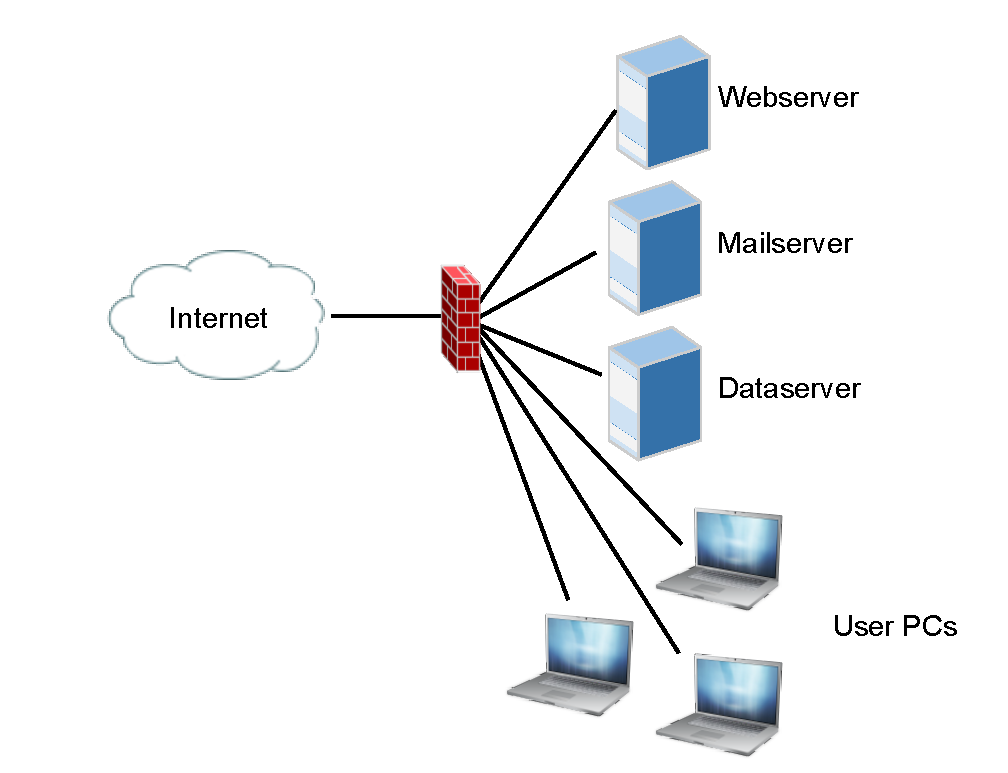
\includegraphics[width=0.6\textwidth]{images/old_system.pdf}  
  \caption{Diagram of the status quo.}
  \label{oldsystem}
\end{figure}

Our task is to design and implement a certificate authority (CA) that provides the employees with digital certificates that will be used to encrypt and authenticate the previously mentioned email conversations.\newline
The created CA should withstand targeted attacks and integrate into the current system. To authenticate employees so that they can create and use certificates, the existing user database should be used. To guarantee the security of the newly built infrastructure, the old system also has to undergo certain changes. We will introduce a new level of isolation for critical systems and put systems that do not have to be accessed directly by users in a separate zone, so that they can not be reached directly. The design of the system will be evaluated in detail in the following sections. An overview of the proposed system is shown in Figure \ref{newoverview}.

\begin{figure}[H]
  \centering
    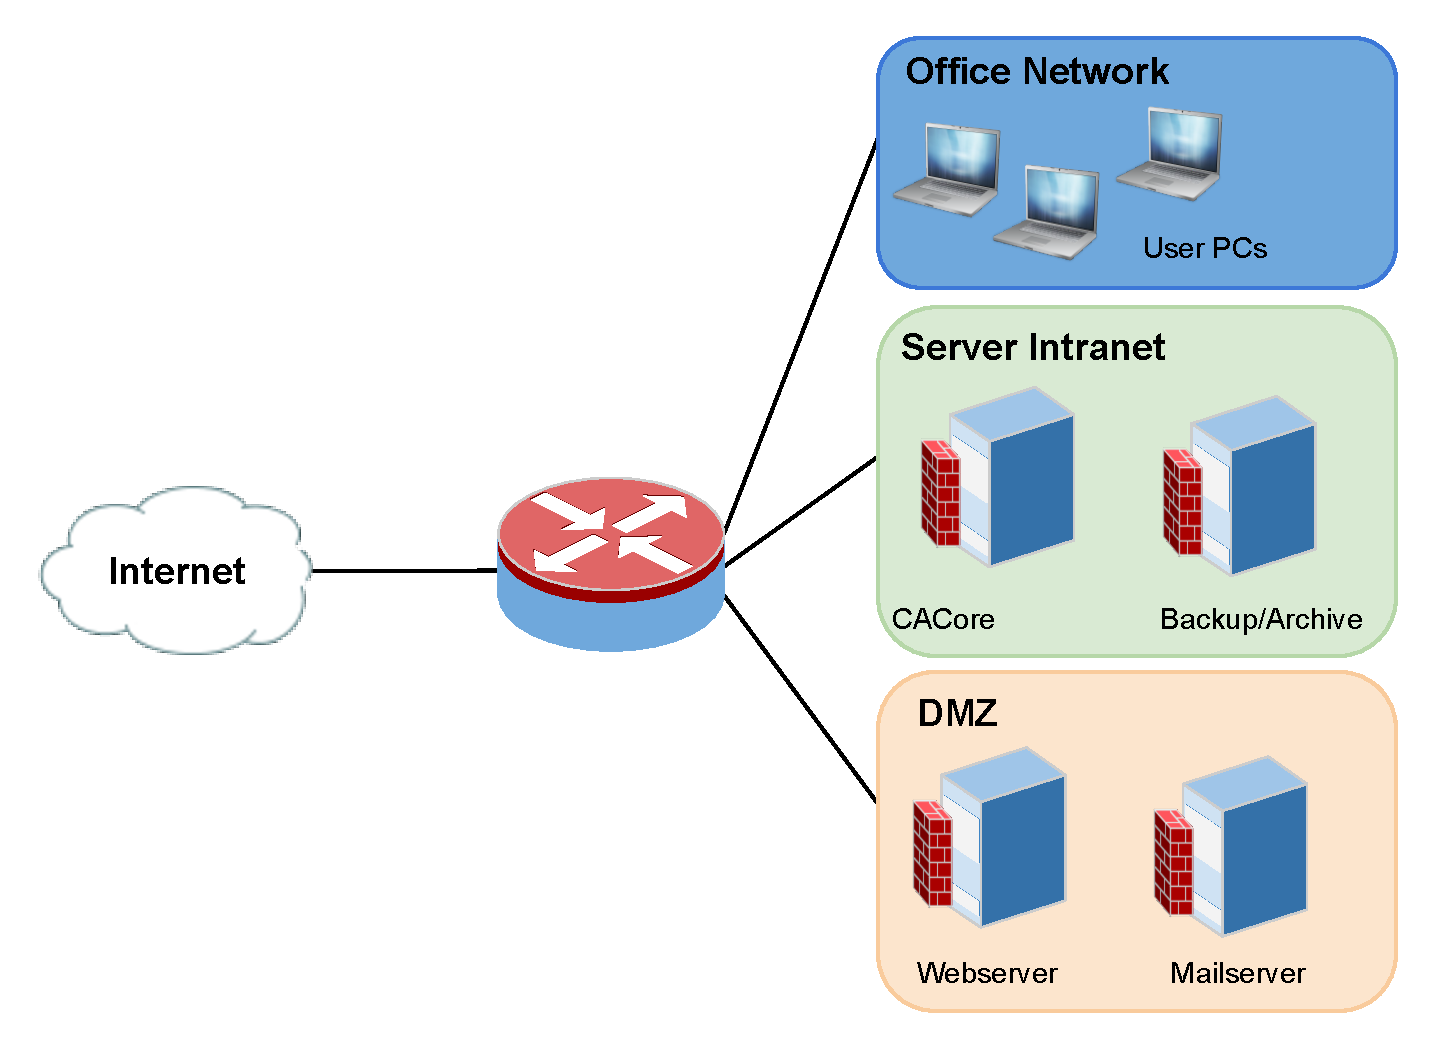
\includegraphics[width=0.6\textwidth]{images/new_overview.pdf}  
  \caption{Overview of the proposed system.}
  \label{newoverview}
\end{figure}

\section{System overview}
To use the newly developed CA's features, an employee connects to a website and authenticates himself with his credentials that are stored in the preexisting database. Afterwards he then can issue a new certificate carrying the user's data or revoke existing certificates that belong to his account. When at least one certificate is obtained, it is also possible to authenticate with said certificate. Even though a regular user only has to interact with the just described web interface, there is more to the system than that. A separate server is responsible for the process of actually issuing and revoking the certificates in compliance with the information stored in the database. The database could actually remain on a different instance, but for reasons of simplicity and since the company is small, we installed the database on the same server as the CA core which implements the previously described functionality of issuing, verifying and revoking certificates. To prevent loss of data, ensure key recovery and auditability on the system in general, we implement a backup solution as well as a logging system and a key archive. These are all systems that do not need regular and close interaction with users or even system-administrators. Because of that, we decided to locate them together on their own, separate backup and archive server.\newline
Since the user only interacts with the web interface which is publicly accessible, this is also the most exposed part of the system. We do not want it in close proximity of the most valuable part of the system, the core CA. We therefore set up a special demilitarized zone (DMZ) in which we place systems and functionality that has to be accessed from the outside. Every other functionality and system is not accessible from the outside and is placed in another zone.\newline
Figure \ref{systemoverview} shows the Webserver placed in the DMZ, the Core CA as well as the Backup/Archive server in an internal server zone.

\begin{figure}[H]
  \centering
    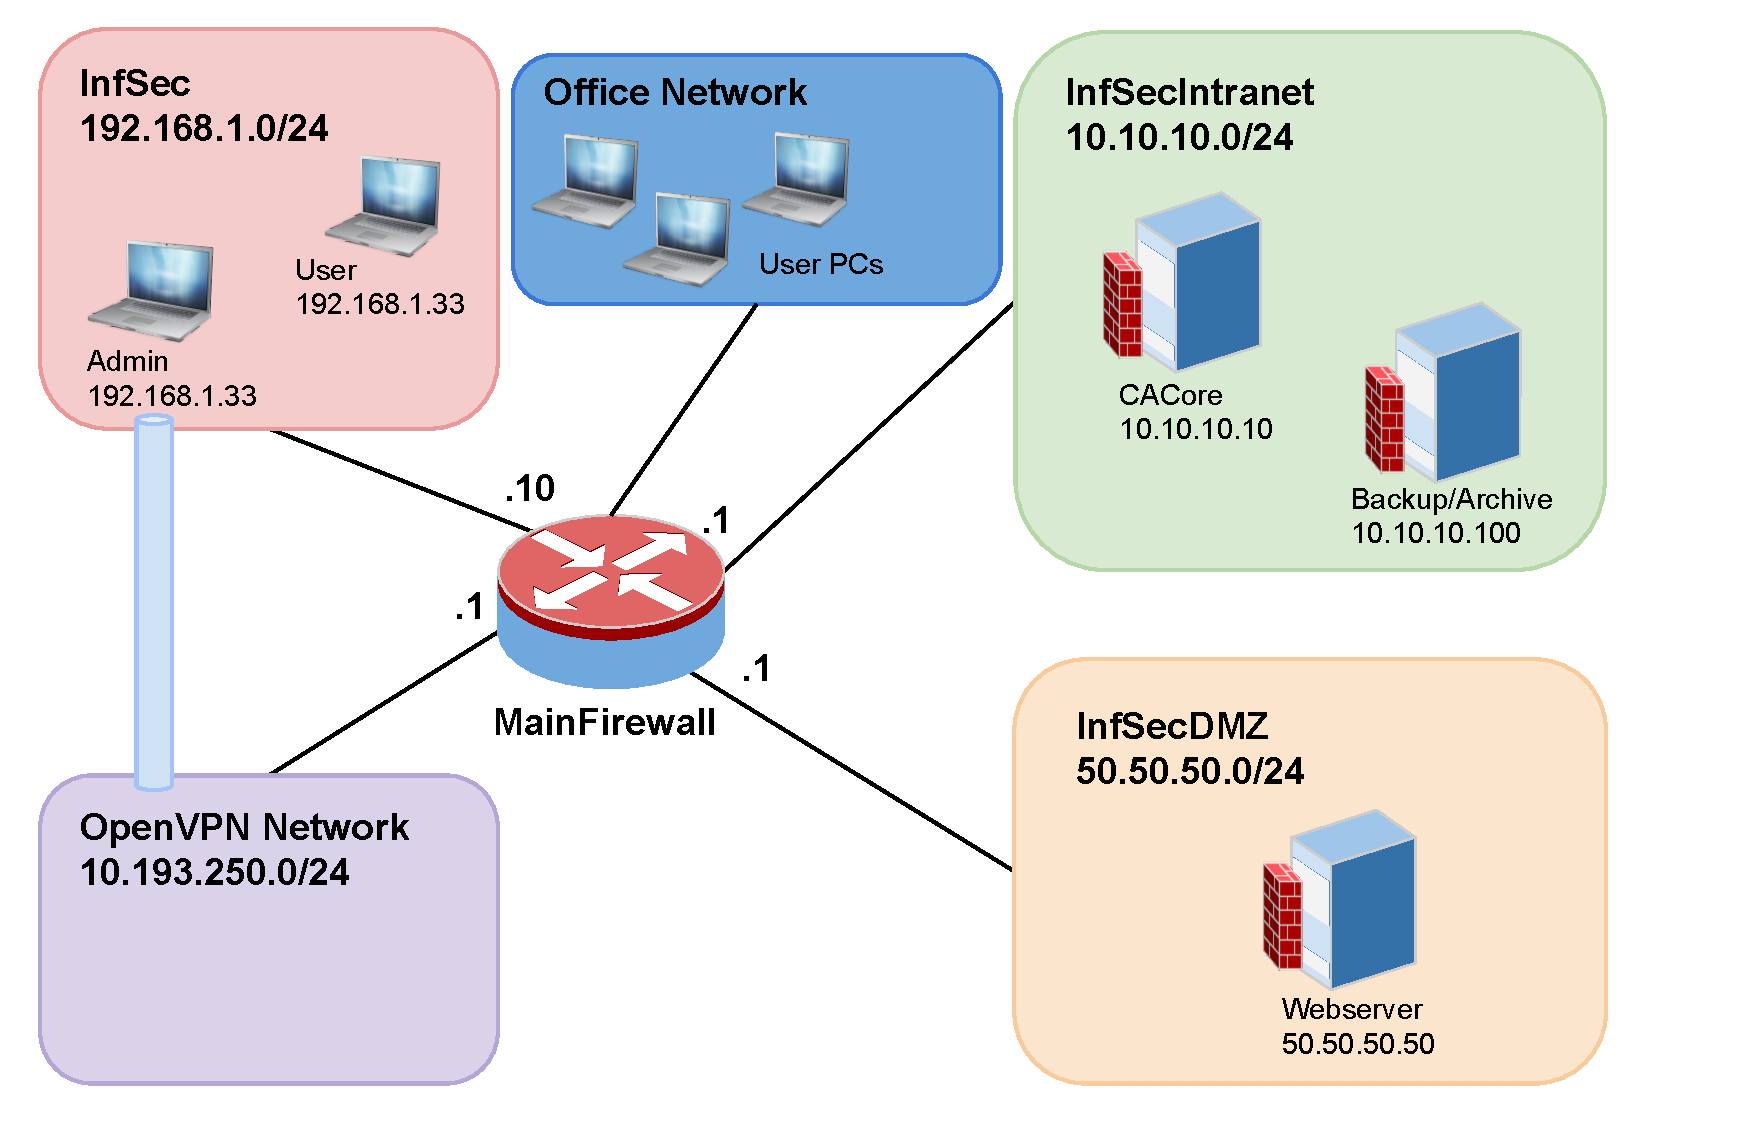
\includegraphics[width=0.6\textwidth]{images/system_overview_new.pdf}  
  \caption{More detailed overview of the proposed system.}
  \label{systemoverview}
\end{figure}

All personal machines of the employees of iMovies are also in their own zone. This is shown in Figure \ref{systemoverview} but will not be elaborated any further in this report, as the topic of the project is to implement a certificate authority.\newline
To allow system-administrators to access all systems remotely, we provide a VPN that allows every system-administrator to access all of the different network zones from a remote workstation.

We proceed with more detailed descriptions of the functionalities of the system and their implementation with special regard to security.

\section{Requirements elicitation and system functionality}
In this section we list the requirements and the functionalities of the proposed system. We first look at the functional requirements and afterwards give an insight into the non functional requirements. We cover security requirements as a separate unit, since we want to emphasize the importance of them to the certificate authority system.

\subsection{Functional requirements}
We first list the functional requirements we extracted from the assignment we got to implement this system. From this these requirements we conclude general use cases of the system and will also give an insight in possible misuse cases.

\begin{description}
\item[User Interface: ]
A simple web interface that allows each user to log in either with his credentials from the legacy MySQL database, or one of his previously generated certificate and private key combinations.
Once logged in the user can view his information (last name, first name and email address), change his password and update his information (last name, first name and email address).
Additionally it is possible for the user to request the system to issue a new certificate (based on his possibly changed credentials) and download the certificate with the newly generated private key in PKCS\#12 format.

\item[Administration Interface: ]
A simple web interface where CA administrators can consult the current CA state after a login process which requires the CA administrators to authenticate themselves with their certificate. This includes the number of issued certificates, the number of revoked certificates and the current serial number.

\item[Certificate Issuing and Revocation: ]
The CA offers an interface that allows other systems to
\begin{itemize}
\item Generate new public/private key pairs.
\item Generate a certificate that ties a public key to a user's credentials (first and last names and his email address) and sign this certificate with the CA's key.
\item Revoke a previously signed certificate.
\item Get a list that contains all revoked certificates (Certificate revocation list).
\end{itemize}

\item[Key Backup: ]
To prevent the loss of any information, that was encrypted with an issued certificate, every issued certificate and the according private key are archived.

\item[System Administration and Maintenance: ]
Each server is remotely accessible for the system administrator. In addition to this, all the configuration files of all machines that are part of the systems as well as the log entries that were created are stored on the backup server.
\end{description}

\subsubsection{Use cases}
Figure \ref{usecase} shows a graphical representation of the use cases. Additionally we will go over every use case individually and offer a short description for it.

\begin{figure}[H]
  \centering
    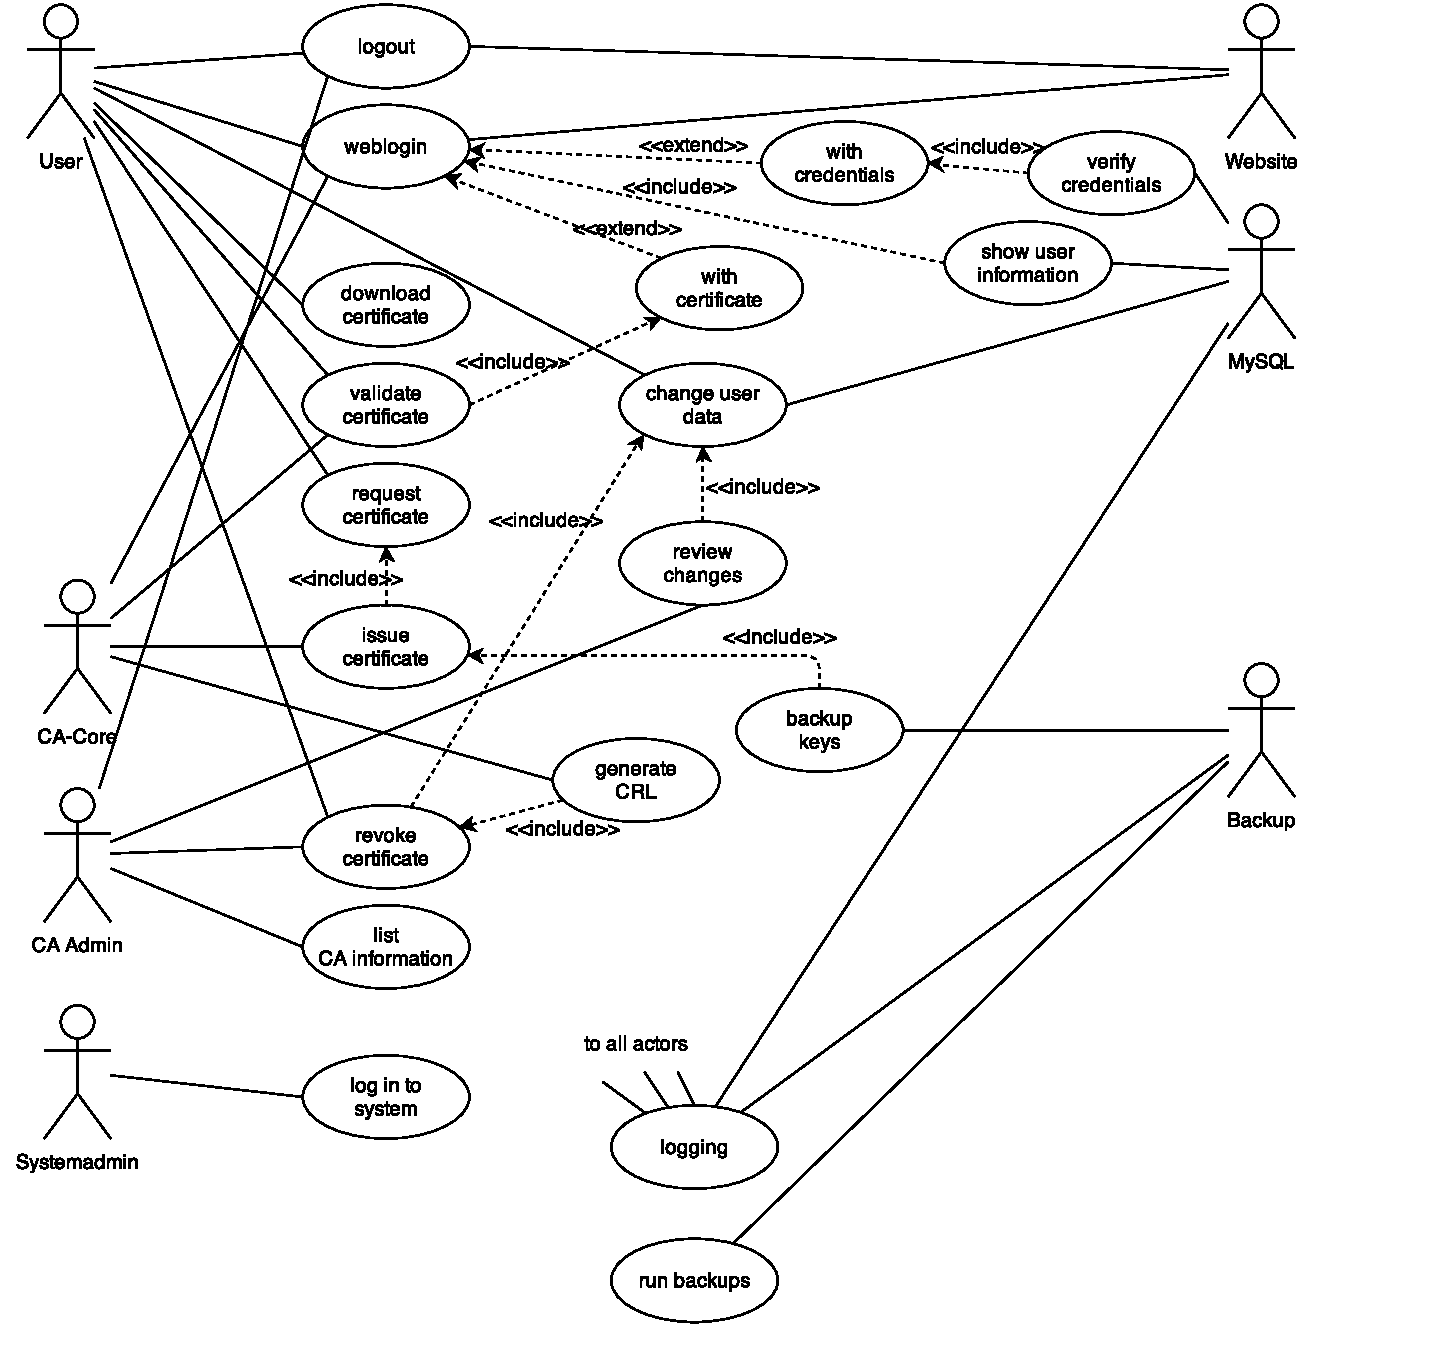
\includegraphics[width=0.7\textwidth]{images/final_usecases.pdf}  
  \caption{Use cases of the proposed system.}
  \label{usecase}
\end{figure}

We first identify the participating roles:
\begin{itemize}
\item User (The employee who uses the web interface to view/change user data, issue, verify, download, revoke certificates)
\item CA Administrator (Administrator who has access to certain CA information)
\item System Administrator (Administrator who can access all systems remotely)
\item Website/Webinterface (Displays information to users and CA Administrators)
\item Core CA (Issues, stores, revokes, verifies certificates)
\item Database (Stores user information)
\item Backup/Archive (Stores certificates, private keys, logging information, backed up configurations)
\end{itemize}
We now list the use cases of these roles:
\begin{description}
\item[Web login ] User logs onto the webserver with his credentials or a certificate.
\item[With certificate ] Login by presenting a certificate.
\item[With credentials ] Login by presenting user name and password.
\item[Verify credentials ] Presented credentials get verified against the information stored in the database (RPC call to CA Core).
\item[Validate certificate ] The presented certificate gets verified. CA Core ensures that it is a proper certificate and not yet revoked or expired/not yet valid.
\item[Show user information ] The user information (not including the user's password) stored in the database is displayed to the user (RPC call to the database).
\item[Change user data ] The user changes any of the information stored (not including his username) in the database.
\item[Review user data changes ] If a user changes information other than the password, the changes have to be reviewed by the CA Administrator before writing them to the database and all the users certificates get revoked if the change is accepted.
\item[Request certificate ] A user sends a request for a new certificate (RPC call to CA Core).
\item[Issue certificate ] The CA Core issues a new certificate for the user who requested it. The certificate and the private key get archived.
\item[Download certificate ] The user can download its newly generated certificate and his private key.
\item[Backup keys ] After creating a new certificate, the CA Core stores the new certificate and the according private key on the backup/archive server. 
\item[Revoke certificate ] A user or the CA Administrator set a certificate for revocation. (RPC call to CA Core).
\item[Generate CRL ] When revoking a certificate, the CA Core generates a new or updates an existing CRL.
\item[List CA information ] When a CA Administrator is logged in, his web interface displays the number of issued certificates, the number of revoked certificates and the current serial number.
\item[System login ] The System Administrator remotely logs into one of the running system and can get root access.
\item[Logging ] Each system automatically sends logging information of the system and the interactions with the system to the backup/archive server.
\item[Run backups ] The backup server periodically runs backups to collect the configurations of the other systems.
\item[Logout ] CA administrator and users that are logged in, can log out, which causes a new login prompt when visiting the site again.
\end{description}

\subsubsection{Misuse cases}
Figure \ref{misusecase} shows the misuse cases and also additional use cases that prevent this misuse cases in a graphical manner. We also list each misuse case individually with a short description.
\begin{figure}[H]
  \centering
    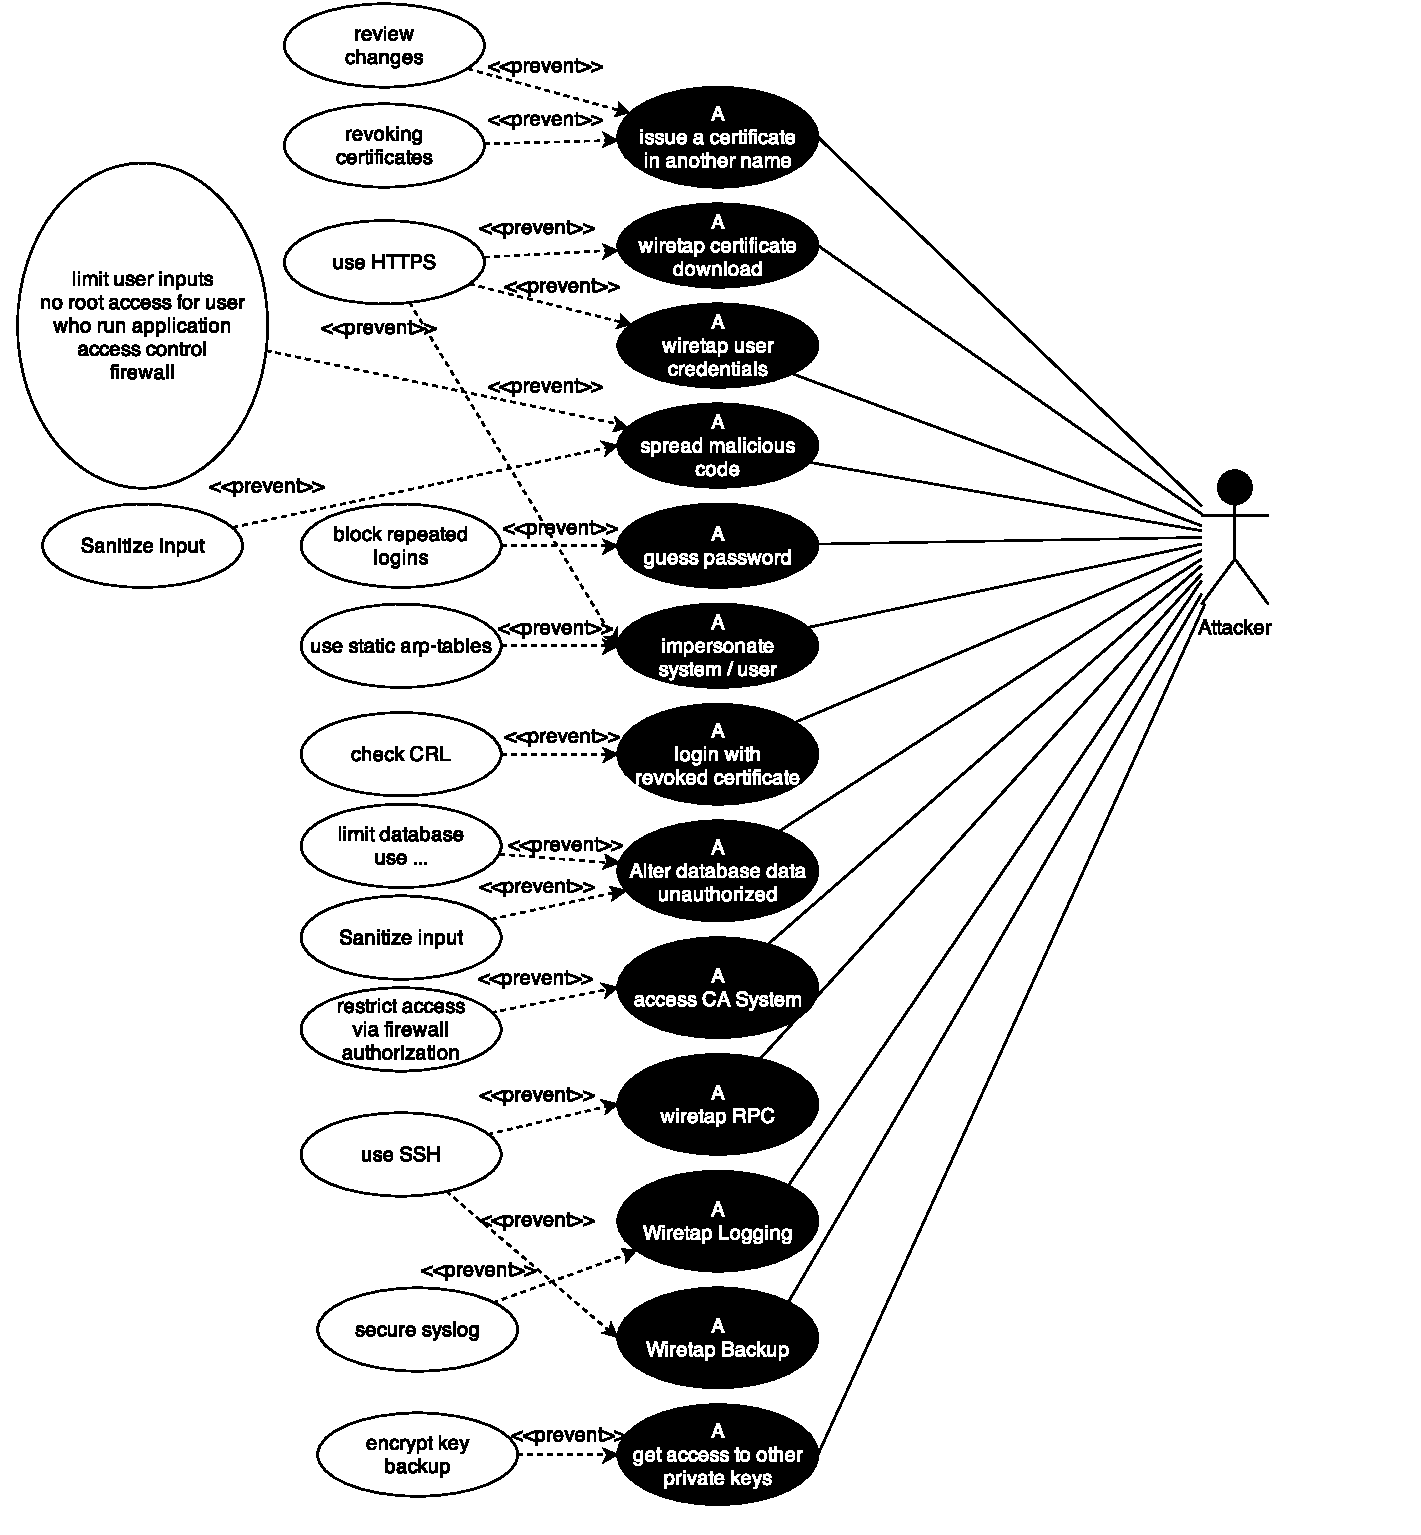
\includegraphics[width=0.7\textwidth]{images/misusediagram.pdf}  
  \caption{Misuse cases and additional use cases of the proposed system.}
  \label{misusecase}
\end{figure}

We first identify the participating roles:
\begin{itemize}
\item Threat agent (The attacker which can be an outsider as well as an misbehaving employee)
\end{itemize}
We now list the misuse cases of these roles as well as the preventing use cases:
\begin{description}
\item[Issue certificate in another name ] The attacker is able to alter his information and then issue a certificate with this information. This gets prevented by the CA Administrator reviewing changes other than to the password and revoking all its issued certificates.
\item[Wiretap certificate download ] The attacker can obtain a copy of the certificate/private key pair of a user. This is prevented with enforcing HTTPS when connecting to the webservice.
\item[Wiretap user credentials ] The username and password get obtained by the attacker during transmission. This is prevented with enforcing HTTPS when connecting to the webservice. For system administrator credentials, use SSH and VPN to connect to remote systems.
\item[Guess password ] With multiple guesses, the attacker can bruteforce the password. To prevent this, limit the number of times a password for a given user can be tried.
\item[Impersonate system/user ] An attacker can spooth and poison communication mechanisms to impersonate a certain role. Use HTTPS and SSH to prevent this. In the infrastructure controlled by iMovies, use static ARP tables to prevent ARP poisoning.
\item[Login with revoked certificate ] The attacker may get access to the system with presenting an invalid certificate. To prevent this, always check the CRL.
\item[Alter database date unauthorized ] An attacker alters data in the database that does not belong to him. To prevent this, one can sanitize the input, review all changes to the database by the CA Administrator and restrict the database user to only the functionality he needs.
\item[Access systems ] The attacker can log in to the server systems. This is prevented by enforcing access control, only allowing certain traffic through the firewall and onto the system.
\item[Access other private keys ] The stored private keys in the archive get obtained by the attacker. To prevent this, the private keys are stored encrypted.
\item[Wiretap RPC ] An attacker obtains information transmitted between the webserver and the CA Core. To prevent this, the RPC traffic is tunneled via SSH.
\item[Wiretap logging ] The logging information from the servers and applications sent to the backup server gets obtained by the attacker. To prevent this, secure syslog is used which uses an SSH tunnel.
\item[Wiretap backup ] The attacker obtains system and configuration information by intercepting the backup transmission. SSH is used for backup to prevent this.
\item[Running malicious code ] An attacker is able to run malicious code on one of the systems. To prevent this, the users executing this systems have limited rights, strong access controls are implemented and input is sanitized.
\end{description}

\subsection{Non functional requirements}
The following list specifies non functional requirements gathered during the analysis.
\begin{itemize}
\item For the user database, the legacy MySQL database has to be used.
\item The schema of the legacy database can not be modified
\item New certificates and their private key are issued in the PKCS\#12 format.
\item Users with a valid certificate can authenticate themselves over SSL/TLS to the website using the certificate.
\end{itemize}

\subsection{Security requirements}
Since the system is developed to improve the general security of the communication between employees, we treat security requirements in a separate section. The following list is compiled from the initial assignment as well as from issues that arise from the misuse case diagram.
\begin{itemize}
\item Access control to CA Core functionality and data.
\item Secrecy and integrity of private keys in the archive.
\item Integrity, non-repudiation and accountability of log files on the backup server.
\item Secrecy and integrity of the user data stored in the database.
\item Access control on all systems.
\item Confidentiality, integrity and authenticity with regards to key transport.
\item Secrecy and integrity of CA Core data during processing and transport.
\end{itemize}

\section{Components and Subsystems}
\begin{figure}[H]
  \centering
    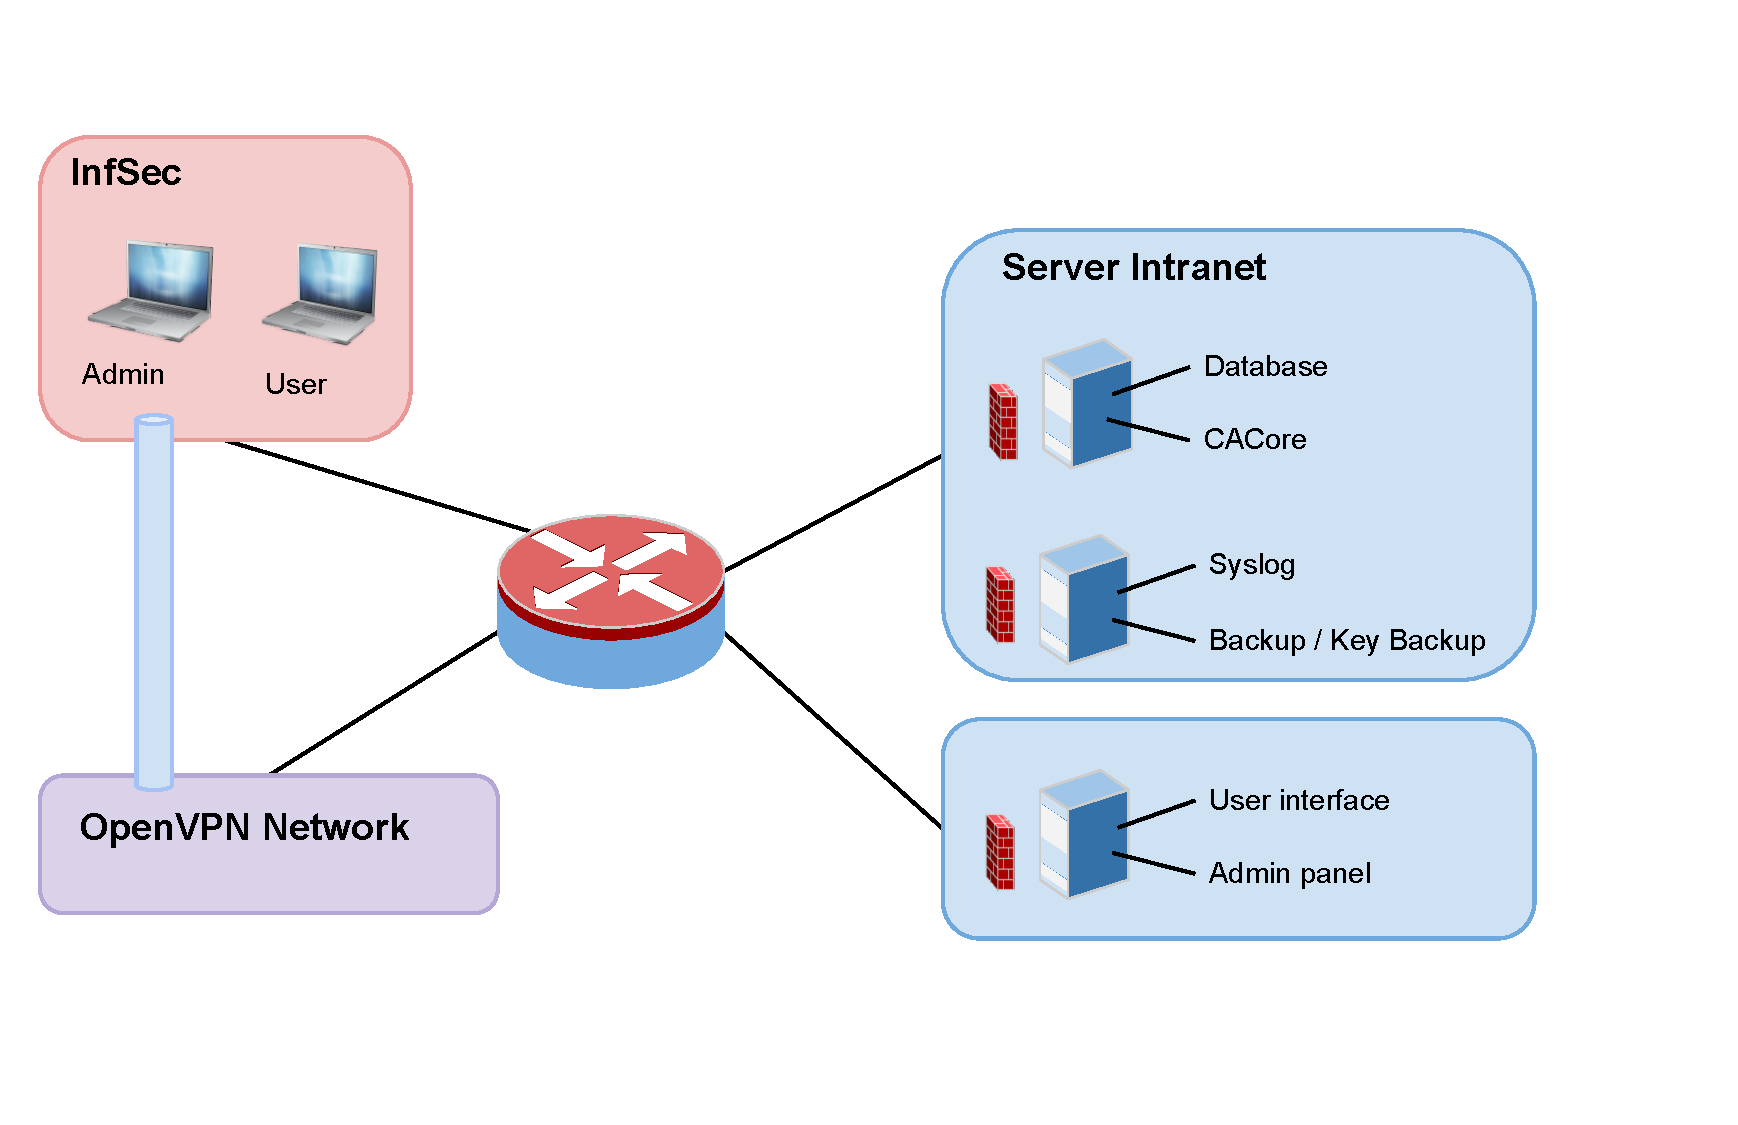
\includegraphics[width=0.6\textwidth]{images/system_components.pdf}  
  \caption{Components of the proposed system.}
  \label{systemcomponents}
\end{figure}

\subsection{Platforms}
The components (as depicted in Figure \ref{systemcomponents}) are as follows:
\begin{description}
\item[Main Firewall ] A software firewall based on Linux (IPCop) that divides the iMovies network into the zones DMZ, internal server network, office network and the internet. The firewall functions as a VPN endpoint for remote administrative access and restricts traffic between the subdivided networks according to a security policy described later.

\item[Web Server ] A Linux machine running Debian 7.2. It hosts the website for the user web interface and the administrative panel. The web server is located within the DMZ, a local iptables firewall allows only HTTPS connections to the outside and SSH connections to the firewall for administration, to the CA Core for secure RPC calls and to the backup server for secure backup and syslog.

\item[CA Core Server ] A Linux machine running Debian 7.2. It hosts the logic for issuing, verifying and revoking certificates as well as the legacy MyQSL database. The server is located within the internal server network, a local iptables firewall allows only SSH connections to the firewall for administration, to the web server for secure RPC calls and to the backup server for secure backup, syslog and key backup.

\item[Backup/Archive Server ] A Linux machine running Debian 7.2. It hosts a syslog server, the logic for periodic backups and storage for encrypted key backup. The server is located within the internal server network, a local iptables firewall allows only SSH connections to the firewall for administration, to the web server and CA Core server for secure backup, syslog and key backup.

\item[Offsite Backup ] Backups of all platforms that is stored on high volume and long living storage media (for example tapes). The media are stored in an highly secure off-site location (for example a bank vault). This is not implemented in the project but would be highly advisable in practice.
\end{description}

\subsection{Applications}

\begin{description}
\item[User Web Interface ] Web application, developed in python running on nginx on the web server that allows the user to issue, verify and revoke certificates as well as view and alter user data. The website interacts with the CA Core via RPC calls.

\item[Administration Panel ] Web application, developed in python running on nginx on the web server that allows the CA Administrator to review user changes and display information about the CAs status. The website interacts with the CA Core via RPC calls.

\item[Legacy DB ] MySQL database with the legacy schema. Running on the CA Core server.

\item[CA Core ] Application using the OpenSSL library that provides basic interfaces to create new key pairs, sign existing key pairs and revoke certificates. Running on the CA-Core server,  interacting with the web server via RPC calls and backing up private keys on the archive server via SSH.

\item[CA Core Storage ] A database that is used by the CA Core to store certain data relevant to the CA Core application. Running on the CA Core server.

\item[Archive] Storage for encrypted public keys and certificates on the Backup/Archive server

\item[Backup ] A script that collects and stores multiple backups from all other servers. This includes configuration files and other important data. It runs on the Backup/Archive server.

\item[Syslog ] A syslog server that receives logging data via SSH tunnel from the other servers, running on the Backup/Archive server.
\end{description}

\subsection{Data}
\begin{description}
\item[User Information ] Basic information according to the schema of the legacy database. This includes the users username, his first and last name, his email address and a hash of his password. This information is stored in the legacy database.

\item[Key Pairs ] Consist of a private key and the according public key that the CA Core generates on request. They are stored permanently in the archive and can be downloaded once immediately after the creation by the user. It is important, that the CA Core destroys his record of the private key as soon as possible.

\item[Certificates ] A certificate that is signed by the CA Core. It is also stored in the archive and additionally also in the CA Storage (to allow certificates to be revoked).

\item[Certificate Revocation List ] A list of certificates, that have been revoked by the CA Core. Stored on the CA Core server and signed by the CA Core.

\item[Local Users ] Credentials, that are used for system administration and communication between the components of the system. Individual to each system.

\item[Configuration Files ] Configuration files define the configuration of a given system. They are in place at the system in question and backed up to the Backup/Archive server.

\item[Log Files ] Log files generated by systems and applications. Stored on the Backup/Archive server.

\item[Master Key ] Master private key to decrypt the encrypted certificate/private key pairs that were generated on request. Stored in multiple high security offline locations (for example a bank vault).
\end{description}

\subsection{Interfaces}
\begin{description}
\item[User Web Interface ]
Offers a user to access his information and certificates. It also allows a user to generate new keys and certificates for those keys. This information can only be accessed when the user authenticates himself with his credentials or a client side certificate.

\item[Administration Web Interface ]
Offers the CA administrator to access information about the certificate authority state. This information can only be accessed when the administrator authenticates himself with a client side certificate.

\item[Legacy DB Interface ]
Offers the functionality to ask for, alter and insert information to and from the database.

\item[CA Core Interface ]
Gets accessed via a RPC to offer the functionality to issue, revoke and verify certificates.

\item[Backup/Archive Interface ]
Implements syslog functionality to provide a syslog endpoint as well as storage for key and configuration backup.
\end{description}

\section{Implementation}
This section describes the implementation of our hardware and software with an emphasis on the security measures installed.
\begin{description}
\item[Main Firewall ] The Main Firewall is a software firewall running the IPCop Linux. It functions as a firewall as well as a router and divides the network into the sections DMZ, internal server network, office network (which is not implemented here), internet and VPN network. This minimizes the exposure of the system\footnote{Basin, Schaller, Schläpfer: Applied Information Security, Principle 1.3.4: Minimize exposure}
 under the assumption that all external systems are insecure\footnote{NIST Special Publication 800-27 Rev A: Engineering Principles for Information Technology Security, Principle 6 \& 20: Assume external systems are insecure \& Isolate public access}, since we separating our core functionalities from the part that is publicly accessible. The routes to the known hardware of the iMovies infrastructure are statically assigned as well as the ARP tables to prevent poisoning. The firewall maintains a VPN using OpenVPN to allow remote access to the VPN network. Remote access to the firewall is possible via SSH using OpenSSH\footnote{NIST Special Publication 800-27 Rev A: Engineering Principles for Information Technology Security, Principle 12: Base security on open standards} out of the VPN network or via webinterface from address 10.10.10.33 from within the internal server network. \newline
The firewall implements several rules on how traffic is allowed to flow between those networks. By default all traffic is denied and silently dropped at the firewall. The following list shows the allowed exceptions: \newline
\begin{tabular}{p{2.5cm} c l p{4cm}}
Source & Protocol & Destination & Description\\
\cline{1-4}
Webserver & HTTP(S) (443/80) & Internet & Allow secure webtraffic from the webserver (HTTP redirected to HTTPS)\\
\cline{1-4}
Internet & HTTP(S) (443/80) & Webserver & Allow secure webtraffic to the webserver (HTTP redirected to HTTPS)\\
\cline{1-4}
10.10.10.33 & IPCop HTTPS (8023) & MainFirewall & Allow the use of the webinterface\\
\cline{1-4}
OpenVPN network & IPCop SSH (8022) & MainFirewall & Allow remote administrative access\\
\cline{1-4}
BackupServer & IPCop SSH (8022) & MainFirewall & Allow backup\\
\cline{1-4}
OpenVPN network & SSH (22) & Backupserver & Allow remote administrative access \\
\cline{1-4}
OpenVPN network & SSH (22) & CACore & Allow remote administrative access \\
\cline{1-4}
OpenVPN network & SSH (22) & Webserver & Allow remote administrative access \\
\cline{1-4}
Backupserver & SSH (22) & Webserver & Allow backup and tunneled logging\\
\cline{1-4}
Webserver & SSH (22) & CACore & Allow tunneled RPC calls\\
\cline{1-4}
CACore & SSH (22) & Webserver & Allow tunneled RPC calls \\
\end{tabular}

\item[Servers in general ] We deploy three servers, the web server, the CA Core server and the Backup/Archive server. All servers are running debian in version 7.2. They have three users, root, an admin and an operational user. The operational user is not in the sudoers list and cannot get root access and should therefore be used to run the applications\footnote{NIST Special Publication 800-27 Rev A: Engineering Principles for Information Technology Security, Principle 26: Implement least privilege}. We deactivated su and only allow sudo. Per default we deny all access via PAM (the Pluggable Authentication Modules). We ensure that the root user can only login locally and disable remote login. Failed login attempts get logged and automatically transmitted to the collected logfiles located on the Backup/Archive server. To prevent poisoning, we fix the ARP tables with the MAC addresses of all interacting systems. \newline
SSH is used for various interactions. We only allow the admin user and the operational user to have SSH access. With the help of sshguard we introduce a exponential time delay after three failed login attempts by implementing temporary rules to the local iptables.\newline
Each server has a local firewall based on iptables which blocks all connections by default\footnote{NIST Special Publication 800-27 Rev A: Engineering Principles for Information Technology Security, Principle 6 \& 20: Assume external systems are insecure \& Isolate public access}. The exceptions are specific to the server and listed in their detailed implementing description.\newline
On the servers, the number of running processes is kept to a minimum, especially processes with network capabilities. With the help of the debian harden package, all unnecessary packages like telnet were removed. The services running on every system are sshd and a status demon. The status demon listens for pyRPC and when connected gives information about the status (total load and free memory) of the system. This is used for external administrators without SSH access. Some systems run additional services which are specified later. 

\item[Webserver ] The basic setup is as described in {\bfseries servers in general}. As the webserver needs additional functionality for running the websites and interacting with the CA Core, some more details have to be provided.\newline
The HTTP daemon used is nginx which was modified to only accept HTTPS requests, meaning redirecting HTTP requests to HTTPS.\newline
We modified the nginx\footnote{nginx-1.4.4, http://nginx.org} configuration file in such a way, that the HTTPD does not leak it's version string in any of the error pages or in the Server header of HTTP responses. Additionally we used several configuration options to reduce the size of different buffers that nginx uses internally for client connections to reduce the risk of buffer overflows.\footnote{Basin, Schaller, Schläpfer: Applied Information Security, Principle 1.3.4: Minimize exposure}
\newline
To reduce the effectiveness of small distributed denial of service attacks (DDOS attacks) we reduced the default timeouts to prevent single clients to freeze the HTTPD by keeping alive a huge number of simultaneous connections and not sending any data. This is a trade-off because client on a very slow connection wont be able to access the webserver. This does not concern us because our use case does not involve connections from very remote places via very slow connections (like satellite uplinks or similar connections). Additional methods to prevent or reduce the effectiveness of larger DDOS attacks include hardware solutions and third party services like Cloudflare or Dragonara. These solutions were not evaluated because they are not in the scope of this report.\newline
To detect potential attacks we use the built in logging facilities of nginx that enable us to store certain information (like the IP address, the HTTP verb or the URL) of every HTTP requests that hits the server. This would enable us to use an intrusion detection system to detect any kind of abnormal activity\footnote{Basin, Schaller, Schläpfer: Applied Information Security, Principle 1.3.10: Log relevant systems}
. At the moment we are not using such a system.\newline
The two applications, the user web interface and the admin panel were developed in python. Both applications were implemented using a python web micro-framework called Flask. This open source solution provides us with the tools to rapidly develop simple and secure web applications.\newline
To prevent cross-site request forgery (CSRF) attacks we are using the CRSF token provided by the flask framework\footnote{flask-0.10, http://flask.pocoo.org} and the user inputs are sanitized in flask automatically to render cross-side script (XSS) attacks impossible.\newline
Data between the web applications and the CA-Core backend is exchanged with a python RPC library called Pyro4. Pyro4 does not support any kind of encryption of the communication. Because of that we tunnel all RPC over a SSH connection to ensure the secrecy and integrity of all calls\footnote{NIST Special Publication 800-27 Rev A: Engineering Principles for Information Technology Security, Principle 9: Protect information while being processed, in transit, and in storage}.

Like all other physicial machines, the webserver has a local iptables firewall which silently drops all packets by default and implements the following exceptions:


\begin{tabular}{p{2.5cm} c l p{4.5cm}}
Source & Protocol & Destination & Description\\
\cline{1-4}
Backupserver & SSH (22) & Webserver & Allow backup and logging\\
\cline{1-4}
OpenVPN network & SSH (22) & Webserver & Allow remote administrative access \\
\cline{1-4}
Internet & HTTP(S) (443/80) & Webserver & Allow secure web traffic (HTTP redirected to HTTPS)\\
\cline{1-4}
CACore & RPC (4444) & Webserver & Allow tunneled RPC call\\
\cline{1-4}
Webserver & HTTP(S) (443/80) & Internet & Allow secure web traffic (HTTP redirected to HTTPS)\\
\cline{1-4}
Webserver & RPC (4444) &  CACore& Allow tunneled RPC call\\
\cline{1-4}
CACore & SSH (22) & Webserver & Allow tunneled RPC call\\
\cline{1-4}
Webserver & SSH (22) & Backupserver & Allow backup and logging\\
\end{tabular}

\item[CA Core ] In addition to the basic setup described in {\bfseries servers in general}, the CA Core server houses the legacy MySQL database and the application that provides the functionality of issuing, verifying and revoking certificates. \newline
The MySQL database grants access to the table iMovies.users via the database user dbuser. This user only has limited rights, namely he can INSERT, SELECT and UPDATE\footnote{NIST Special Publication 800-27 Rev A: Engineering Principles for Information Technology Security, Principle 26: Implement least privilege}
. There is no need for encrypting SQL traffic, as the database is on the same host as its consumer.\newline
The application which implements the certificate authority (CA) functionality is written in python and uses the pyOpenSSL module which is a python wrapper for the openssl library. It is used to create, revoke and sign certificates. In addition to that, another openssl wrapping library called m2crypto is used to verify if a given certificate is valid because pyOpenSSL does not provide this functionality\footnote{NIST Special Publication 800-27 Rev A: Engineering Principles for Information Technology Security, Principle 8: Implement tailored system security measures to meet organizational security
goals}.\newline
To query the legacy MySQL database, the CA application uses a python object relational mapper called SQLAlchemy. This enables us to query the database without writing our own SQL statements. In addition to that SQLAlchemy automatically escapes user input in all statements which serves as protection against SQL injection attacks. Internally SQLAlchemy uses MySQLdb, a python interface to MySQL databases.\newline
As previously mentioned in the {\bfseries Webserver} item, the CA application offers a RPC endpoint that is implemented using the Pyro4 middleware.\newline
To ensure the secrecy of the generated private keys, the application discards the keys after it sent them to the web application that requested the creation.\newline
The application allows normal users to log in with a user/password combination that is stored in the legacy database or a previously generated and not revoked private key/certificate pair. A successful login starts a new session that is attached to the user that signed in. Without a valid session, the CA application does not allow to create new certificates. A session becomes invalid after 30 minutes without any action. CA administrators can only authenticate themselves with a special CA admin certificate.\newline
After generating a new private key and creating a certificate for the according public key, the CA application stores the private key and the certificate as an encrypted file locally. Once every hour all those key backup files are transferred to the Archive via a secure SSH connection. They can only be decrypted with a RSA private key that is stored in multiple high security offline locations (for example a vault in a Swiss bank) and can not be accessed by a system administrator\footnote{NIST Special Publication 800-27 Rev A: Engineering Principles for Information Technology Security, Principle 9 \& 26: Protect information while being processed, in transit, and in storage \& Implement least privilege}.\newline
The CA application implements fine grained logging using three different log levels called debug, info and error. Messages logged on the debug level are discarded immediately on any production system. Info and error messages are sent to the Backup automatically\footnote{Basin, Schaller, Schläpfer: Applied Information Security, Principle 1.3.10: Log relevant system}.

\begin{tabular}{p{2.5cm} c l p{4.5cm}}
Source & Protocol & Destination & Description\\
\cline{1-4}
Backupserver & SSH (22) & CACore & Allow backup and logging\\
\cline{1-4}
OpenVPN network & SSH (22) & CACore & Allow remote administrative access  \\
\cline{1-4}
Webserver & RPC (4444) & CACore & Allow tunneled RPC call \\
\cline{1-4}
CACore & RPC (4444) & Webserver & Allow tunneled RPC call \\
\cline{1-4}
CACore & SSH (22) & Backupserver & Allow key backup \\
\cline{1-4}
Webserver & SSH (22) & CACore & Allow tunneled RPC call \\
\cline{1-4}
CACore & SSH (22) & Webserver & Allow tunneled RPC call \\
\end{tabular}


\item[Archive/Backup server ] The functionality this server implements in addition to the basic setup described in {\bfseries servers in general} is storage for the backed up private keys and a script that backs up the configurations of the servers and collects the logging data of the other machines and applications. Backup, logging and key backup is done directly via SSH or via an SSH tunnel.\newline
The local iptables firewall that closes all ports by default implements the following exceptions:

\begin{tabular}{p{2.5cm} c l p{4.5cm}}
Source & Protocol & Destination & Description\\
\cline{1-4}
CACore & SSH (22) & Backupserver & Allow key backup\\
\cline{1-4}
OpenVPN network & SSH (22) &  Backupserver & Allow remote administrative access\\
\cline{1-4}
Backupserver & SSH (22) & CACore & Allow backup\\
\cline{1-4}
Backupserver & SSH (22) & MainFirewall & Allow backup and logging\\
\cline{1-4}
Backupserver & SSH (22) & Webserver & Allow backup and logging\\
\cline{1-4}
\end{tabular}
\end{description}

\section{Operation}
During operation of the system several actions can be performed to keep the system secure and detect misuse or an attack early on.\newline
\begin{description}
\item[Update ] Perform weekly security updates on all production machines. To perform the updates the whole system is shut down for a small period to guarantee that the update can not have any side effects.
\item[Logging ] Evaluate the logs and look for anomalies and unintended patterns.
\item[Audit ] Make sure that the information in the logs can be linked to a specific user and action for accountability.\footnote{NIST Special Publication 800-27 Rev A: Engineering Principles for Information Technology Security, Principle 22 \& 33: Design and implement audit mechanisms to detect unauthorized use and to support incident investigations \& Use unique identities to ensure accountability}
\item[Backup ] Check that the backups work and also check if playing back a backed up configuration would work.
\item[Detection ] Try to detect misuse with monitoring programs. An example would be monitoring overall network traffic which should be fairly low under normal usage or run intrusion detection systems. The installed libraries harden-nids for network intrusion detection and harden-surveillance for network surveillance from the harden package can help with this.
\end{description}

\section{System documentation}
This section is in some sense a summary of the previous ones with some additional information about the systems like usernames, passwords, IP addresses, virtual network names etc. Use this section for administrative purposes of the system.\newline

\subsection{Network diagram}

\begin{figure}[H]
  \centering
    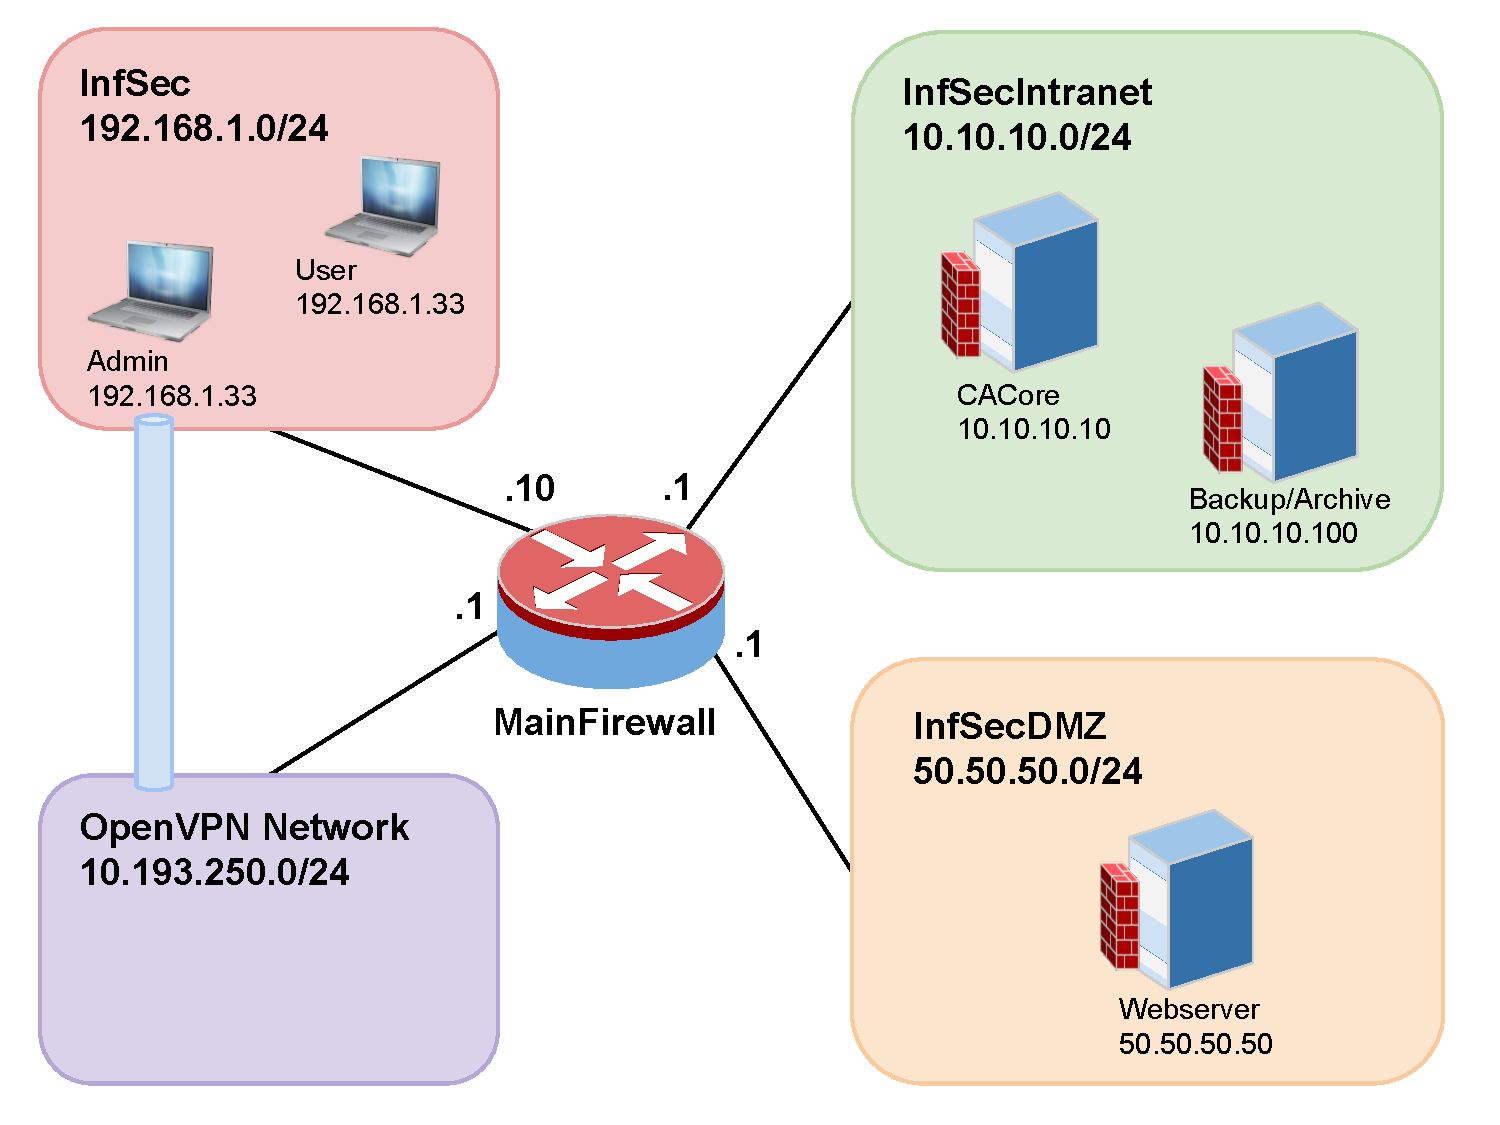
\includegraphics[width=0.8\textwidth]{images/sysseclab_net_diagram.pdf}  
  \caption{Network Diagram}
  \label{netdiag}
\end{figure}

\subsection{Machines}
All servers are equipped with at least one network interface card (NIC) corresponding to the network they are in as shown in Figure \ref{netdiag} and a NAT NIC that can be used for internet access (git, apt-get, etc.). The NAT NIC has to be disabled in production.

\subsubsection{MainFirewall}
\subsubsection*{Accounts \& Passwords}
\begin{multicols}{2}
\begin{description}
\item[admin:] wT7nDB7A7d7V
\item[root:] 5hmAMWxN6uVa
\end{description}
\end{multicols}
\subsubsection*{Installed software}
IPCop
\subsubsection*{User for ssh access}
Accessible only on 10.10.10.1 with port 8022 from 10.10.10.33 (user in InfSecIntranet) or from OpenVPN-Network.\newline
ssh -p 8022 admin@10.10.10.1
\subsubsection*{Additional information}
There is a webinterface on https://10.10.10.1:8023. Only accessible from 10.10.10.33 (user in InfSecIntranet).

\subsubsection{Webserver}
\subsubsection*{Accounts \& Passwords}
\begin{multicols}{2}
\begin{description}
\item[serveruser:] 3FaVLt9RNxLu
\item[root:] cLepMVRq8wDQ
\item[operuser:] KLs3PbjoXu9m
\end{description}
\end{multicols}
operuser cannot use sudo/su and should therefore be used to run the application.
\subsubsection*{Installed software}
Debian, iptables, nginx, python, flask, openSSL, openSSH
\subsubsection*{Running services (lsof -i)}
sshd, nginx
\subsubsection*{User for ssh access}
ssh \{operuser, serveruser\}@50.50.50.50
\subsubsection*{additional information}
SSL signing key for HTTPS: 9klTRxBQcAnM

\subsubsection{CoreCA}
\subsubsection*{Accounts \& Passwords}
\begin{multicols}{2}
\begin{description}
\item[causer:] 9BxkXM5fLLL8
\item[root:] 8kSeddphG6Ac
\item[operuser:] PrCgs5TLqW4f
\item[SSH user web:] xGIv663pLveu
\end{description}
\end{multicols}
operuser cannot use sudo/su and should therefore be used to run the application.
\subsubsection*{Installed software}
Debian, iptables, python, mySQL, openSSL, openSSH
\subsubsection*{Running services (lsof -i)}
sshd, mysql (only localhost)
\subsubsection*{User for ssh access}
ssh \{operuser, causer\}@10.10.10.10
\subsubsection*{additional information}
MySQL root: Cm7NsWBhf52C\newline
MySQL dbuser: Q8mxLsBwTLJi\newline
dbuser is only allowed to INSERT, SELECT, UPDATE the tables iMovies.users, iMovies.sessions, iMovies.admin\_sessions, iMovies.update\_request, iMovies.certificates, thus should be used for connecting to the database.

\subsubsection{Backup/Archive Server}
\subsubsection*{Accounts \& Passwords}
\begin{multicols}{2}
\begin{description}
\item[archiveuser:] 4uMtrPMLxShw
\item[root:] gaBWUt5EH8vU
\item[operuser:] QT5wbxjCN8gG
\item[SSH user core:] f78yefhGm4n4
\item[SSH user web:] 5eK2C131HW41
\end{description}
\end{multicols}
operuser cannot use sudo/su and should therefore be used to run the application.
\subsubsection*{Installed software}
Debian, iptables, openSSH
\subsubsection*{Running services (lsof -i)}
sshd
\subsubsection*{User for ssh access}
ssh \{operuser, archiveuser\}@10.10.10.100

\subsubsection{User}
\subsubsection*{Accounts \& Passwords}
\begin{description}
\item[loginname: administrator username: alice:] alice
\item[loginname/username: alice:] bob
\end{description}
\subsubsection*{additional information}
When running in netwok InfSec, VPN is possible (VPN start script on Desktop):\newline
User administrator/alice has the CA administrator certificate installed.\newline
User administrator/alice has a VPN script on the desktop with which needs to be used for administrative access on the servers.\newline
User bob is a normal client.
\begin{description}
\item[PKCS12 PW:] StgmE58sadQu
\end{description}
When running in netwok InfSecIntranet, firewall web access on https://10.10.10.1:8023


\subsection{Firewall rules}
\subsubsection{MainFirewall}
All connections are closed by default. The following list shows the allowed exceptions:\newline

\begin{tabular}{l c l}
Source & Protocol & Destination \\
\cline{1-3}
Webserver & HTTPS (443) & InfSec \\
\cline{1-3}
InfSec & HTTPS (443) & Webserver \\
\cline{1-3}
10.10.10.33 & IPCop HTTPS (8023) & MainFirewall\\
\cline{1-3}
OpenVPN network & IPCop SSH (8022) & MainFirewall \\
\cline{1-3}
10.10.10.33 & IPCop SSH (8022) & MainFirewall \\
\cline{1-3}
BackupServer & IPCop SSH (8022) & MainFirewall \\
\cline{1-3}
OpenVPN network & SSH (22) & Backupserver \\
\cline{1-3}
OpenVPN network & SSH (22) & CACore \\
\cline{1-3}
OpenVPN network & SSH (22) & Webserver \\
\cline{1-3}
Backupserver & SSH (22) & Webserver \\
\cline{1-3}
Webserver & SSH (22) & CACore \\
\cline{1-3}
CACore & SSH (22) & Webserver \\
\end{tabular}

\subsubsection{Webserver}
All connections are closed by default. The following list shows the allowed exceptions:\newline


\begin{tabular}{c c c}
Source & Protocol & Destination \\
\cline{1-3}
Backupserver & SSH (22) & Webserver \\
\cline{1-3}
OpenVPN network & SSH (22) & Webserver \\
\cline{1-3}
InfSec & HTTPS (443) & Webserver \\
\cline{1-3}
CACore & RPC (4444) & Webserver \\
\cline{1-3}
Webserver & HTTPS (443) &  \\
\cline{1-3}
Webserver & RPC (4444) &  \\
\cline{1-3}
CACore & SSH (22) & Webserver \\
\cline{1-3}
Webserver & SSH (22) &  \\
\end{tabular}

\subsubsection{CoreCA}
All connections are closed by default. The following list shows the allowed exceptions:\newline


\begin{tabular}{c c c}
Source & Protocol & Destination \\
\cline{1-3}
Backupserver & SSH (22) & CACore \\
\cline{1-3}
OpenVPN network & SSH (22) & CACore \\
\cline{1-3}
Webserver & RPC (4444) & CACore \\
\cline{1-3}
CACore & RPC (4444) & Webserver \\
\cline{1-3}
CACore & SSH (22) & Backupserver \\
\cline{1-3}
Webserver & SSH (22) & CACore \\
\cline{1-3}
CACore & SSH (22) & Webserver \\
\end{tabular}

\subsubsection{Backup/Archive Server}
All connections are closed by default. The following list shows the allowed exceptions:\newline


\begin{tabular}{l c l}
Source & Protocol & Destination \\
\cline{1-3}
CACore & SSH (22) & Backupserver \\
\cline{1-3}
OpenVPN network & SSH (22) &  Backupserver\\
\cline{1-3}
Backupserver & SSH (22) & CACore \\
\cline{1-3}
Backupserver & SSH (22) & MainFirewall \\
\cline{1-3}
Backupserver & SSH (22) & Webserver \\
\end{tabular}

\iffalse
\section{Backdoors}

In the following sections we list the backdoors we implemented in our system to grant the possibility to compromise the system to a potential attacker.

\subsection{Easy Backdoor}
The easy backdoor is implemented in the status daemon. We use a known vulnerability in the python pickle marshaller to allow remote code execution\footnote{BlackHat 2011, Marco Slaviero, Sour Pickles: Shellcoding in Python's serialisation format}
.\newline
As we forward all traffic from all remote machines directly over port 4445 and 4446 to the web and core servers the attacker can compromise both systems and get access to the CA key or other confidential data stored on both of those servers. By using additional unpatched bugs or vulnerabilities in other software running on those servers it could be possible to even infiltrate the backup/archive server.

\subsection{Hard Backdoor}
The second backdoor is better hidden. We used the fact, that the python interpreter we use (cPython) looks for previously compiled bytecode for each imported python module in a $.pyc$ file. If a $.pyc$ file exists for a module $.py$ file, the interpreter checks if the timestamp that is included in the $pyc$ $header$ matches the imported $.py$ file and if so it does not recompile the $.py$ file. We use this little known fact to compile a vulnerable $core.py$ file of the Pyro4 RPC middleware into the $core.pyc$ file and restore the original $core.pyc$ header to prevent the python interpreter to recompile the $.pyc$ file.\newline
The actual backdoor in the $core.py$ file checks in each RPC call if the called method matches $credential\_login$ and when it does, it checks if the provided username has a certain prefix. If so, it extracts a filename from the provided username, uses the password as offset $n$ and tries to read the $nth$ bit of the provided file. If the bit is 0 it returns a login error and otherwise a login success message.\newline
Using this technique an attacker can read any file that the core RPC application can read, although in a slow and complicated way. Using an automated script and masking the login attempts with valid logins over a longer period of time, it could be possible to for example read the CA key and therefore compromising the system.
\fi

\chapter{Risk Analysis and Security Measures}
\section{Stakeholders}
The process of protecting email content with certificates for investigative journalism and film making at iMovies involves three stakeholders.
\begin{description}
\item[iMovies] as a company and all its employees who are sending emails encrypted/authenticated by the new CA system. The informant needs to trust the company and all it's employees, that they do not disclose any information about the informant or his statements to the investigated party. To keep a good reputation among potential future informants it is essential that iMovies stays trustworthy.
\item[Informants] are the people who disclose sensitive information about the investigated party. Informants need to trust iMovies to handle the information handed over delicately.
\item[Investigated party] are the people or company that is investigated by iMovies and who's information gets disclosed by the informant. Their goal is to find the informant or the leaked information.
\end{description}
This risk analysis is commissioned by iMovies and hence we consider iMovies point of view when conducting threat and asset analysis.

\section{Information Assets}
In this section we outline the assets of the system, which includes everything that is part of the system and of value to the stakeholder. We treat each asset type (physical objects, logical objects, persons and intangible goods) in it's own section.

\subsection{Physical assets}
\begin{description}
\item[Firewall ] The firewall is located in the locked and air conditioned server room on the first floor of the iMovies office building, that is equipped with an automated fire protection system. It is housed in a separate rack with two redundant power supplies. The state of the firewall can either be up, up and compromised or down. Where up defines working as intended, up an compromised means the firewall is running but there is unauthorized logical or physical access to the system and down describes a non working firewall.
\item[Webserver ] The webserver is located in the locked server room on the first floor of the iMovies office building in a separate rack with two redundant power supplies. Possible states are similar to the firewall.
\item[CA Core server ] The core server is located in the same room as the firewall and the webserver and also has a redundant power supply. It has similar possible states as the firewall.
\item[Archive/Backup server ] The backup server is located in the same room as the firewall, core server and the webserver and also has a redundant power supply. Possible states are similar to the firewall.
\item[Internal network ] The devices in the server room are directly connected to the firewall, the employees work stations are connected to a switch on each floor which has a direct connection to the firewall. Possible states are up, up and compromised, restricted or down. Up is working as defined, up and compromised is up but with unauthorized access to the resource, like eavesdropping, restricted describes a slow or congested network and down is not working at all.
\item[Internet connectivity ] The ISPs modem is directly connected to the firewall and placed in the same rack. The sates are up, restricted or down. Up is working as defined, restricted describes a slow or congested connection and down is not working at all.
\item[Workstations/laptops ] These are the machines the employees are working with. They are located in the office network and as states they have either up, compromised or down. Where up and down simply mean on and off of a functioning machine and compromised describes a virus/malware infected machine.
\end{description}

\subsection{Logical assets}
\subsubsection{Software}
\begin{description}
\item[Workstations/laptops ] Workstations and laptops are running Ubuntu Linux 12.04 LTS. The only used software are an email client and a web browser. The state of all of these software products can either be up-to-date, old and containing known vulnerabilities or exploited. The workstations are accessed by the employees.
\item[Firewall ] The device runs the newest version of IPCop and is updated regularly by the system administrator. The same states as for the workstations can be applied here. The firewall is only accessible by the system administrator.
\item[Webserver ] The server is running the latest stable version of Debian and is updated regularly by the system administrator. The same states as for the workstations can be applied here. The webserver is only accessible by the system administrator.
\item[CA Core server ] For the CA Core server description of the Webserver can be applied.
\item[Web application ] The software is written in python and works in combination with nginx which both run on the webserver. It is the part of the system that interacts with the user and the CA administrator and is an integer part in the process of issuing, verifying, downloading and revoking certificates. The application is a customized product and is maintained and updated by the manufacturer. The system administrator regularly checks for updates for nginx, python and all used python libraries and reports flaws of the web application to the manufacturer. The states of the web application are running, running and compromised or down. Where running is working as intended with up-to-date software and down is not working at all. Running and compromised means the system is working but is not up-to-date, has known vulnerabilities or exploited vulnerabilities. The application is accessible by every employee that has an user account in the legacy database. The application itself runs with a system user that has no administrative right nor can gain them.
\item[Core application ] This software is a customized product written in python and holds the core functionality of the system, issuing, verifying and revoking certificates. It uses the database to identify users and runs on the CA Core server. The system administrator regularly checks the logs and behavior of the application and reports flaws of the application to the manufacturer. The states of the core application are running, running and compromised or down, where running is working as intended with up-to-date software and down is not working at all. Running and compromised means the system is working but is not up-to-date, has known vulnerabilities or exploited vulnerabilities. The application is only accessible by the system administrator and runs with a user that has no administrative rights nor can gain them.
\item[Database ] The database is a legacy product running MySQL. It stores the user data, runs on the CA Core Server and interacts with the core application. The database user can only access the user table and perform only limited operations. Possible states of the database are up, up and compromised or down. Up and compromised in this case means that data in the database was altered without the user knowing.
\item[Archive/Backupserver ] For the Archive/Backupserver description of the Webserver and Firewall can be applied.
\item[Logging script] The logging scrip is running on the Archive/Backupserver and collects logging information from all other physical assets. Only system administrators can access the logged data. The state of the service is either up, up and compromised when logging info is recorded or false information is inserted, or down.
\item[SSH ] The service used for secure communication between different systems which runs on every physical asset. Only administrative and operative users are allowed to use it and only system administrators can change configurations. The associated states are running, running but compromised in the sense of misconfiguration or insecure use or down.
\item[Backup script ] This software runs on the Archive/Backupserver and collects configuration and data from all other physical assets for backup. The application is a customized product and the system administrator regularly checks the logs and behavior of the script and reports flaws to the manufacturer. Running, running compromised or down are the states where running compromised describes a behavior where only partial data gets backed up or the backed up data gets eavesdropped on.
\end{description}

\subsubsection{Information}
\begin{description}
\item[User data ] Defines the user's data associated with a certificate as well as the user's credentials. User data is stored in the legacy MySQL database and accessible by the core application when the corresponding user executes specific commands, as well as by the system administrator. The system administrator however only sees a hashed version of the password. The state space of the user data corresponds to the people who have access to it. For displaying and changing, authorization has to be given. For the password confidentiality is necessary. The states are private when only the user and system administrator (not the password) have access to the data and disclosed when more people then the user have access.
\item[Login credentials ] The login data for the system defined in the physical assets. They are different for every system and should only be known to the system administrator. If this is the case, the state is private and disclosed otherwise.
\item[Private key ] One of the keys that a specific user generated during the creation of the certificate on the CA Core by the core application. The key should only be accessible by the user for which it was generated. Confidentiality of the private key has to be guaranteed at all times. A key therefore has two states, private as intended or disclosed when other people then the user have access to it.
\item[Certificates ] The certificate asset consists of the certificate and the user in the database associated with the certificate. The certificate should be accessible by everybody, but the relation between the user information and the certificate is fixed. If one of the two is edited, the information and because of that the certificate becomes invalid. The states of the assets are therefore valid and invalid.
\item[CRL ] A list of certificates that have been declared invalid, or in other words have been revoked. Availability of this list is essential. The associated states are available and not available.
\item[Logs ] This is the data that describes what happened in all the system. It is stored locally and on the Archive/Backup server. For accountability the logs should not be writable by the system administrator and confidential for other entities. It is also essential that it is not possible to inject any chosen data into the logs. The states are therefore secure, tampered with or disclosed.
\item[Configurations ] Describe the configurations running on the software and physical assets. Confidentiality of these files should be ensured as only system administrators should have access and the configurations should not be tampered with. The states are therefore similar to the ones of the logs.
\item[Key archive ] Each certificate and the according private key that is generated by the core application is encrypted and then transferred to the archive on the backup server in case the private key of a user gets lost. Nobody in the system should have access to a private key that does not belong to him. The key archive encryption key should not be known to people who have access to the system. Confidentiality of this asset is essential. The states are therefore secure or disclosed.
\item[RPC calls ] The information exchanged between the web application and the core application. Authenticity, integrity and confidentiality should be guaranteed at all times, since confidential information like private keys or user passwords are sent. The states of the asset are secure and compromised.
\item[Web sessions ] The session a user has with the web application after a successful login with his credentials or with one of his previously generated certificates. This session should be unique between the web application and the user and should not be reproducible or replayed once the user or the application has closed the session. The states of this asset are established, compromised or closed. Compromised meaning that someone else than the application or the user participates in the session.
\item[Connectivity ] Includes connections within the iMovies physical network hardware, as well as connectivity to the ISP which are both essential for the operation of the certificate authority. Deterioration of the connectivity also deteriorates the service provided. Availability is an essential factor of this asset. The states are up, restricted (only partially functioning) and down.
\item[Tape backup ] The data backed up to the Archive/Backup server periodically gets backed up to tape which is stored in a physically different location than the iMovies offices. Access to this asset should be limited to system administrators. It could also be listed as a physical asset, since it has to be stored in a save physical location like a safe to protect it against theft, unauthorized access and environmental influences. It has two states, safe, when in a secure location or unprotected, everywhere else.
\item[Key archive encryption key] The key that is used to encrypt the private keys for backup. Confidentiality and availability is essential. It should also only be accessed by personnel different from system administrators and stored in a secure location like a bank vault. The states of this assets are secure and disclosed.
\item[CA signing key] The key that is used by the core application to sign the certificates created. The key has to be accessible by to the application on the CA Core server, thus it is accessible for the system administrator. Confidentiality of the key is critical. If the key is leaked outside the iMovies server intranet the system is compromised, since everyone could sign a certificate in the name of iMovies. The states of the key are secure and leaked.
\end{description}
\subsection{Persons}
\begin{description}
\item[User/Employee ] Users of the system are the iMovies employees who are in contact with the informants. They are valuable to the company since their connections usually leave with the employee. They are also a possible source of threats if they misbehave knowingly and try to harm the system or unknowingly when they use the system with an infected computer and thus compromise the system.
\item[CA administrator ] The person in charge of validating user changes other than changes to the password. He also oversees the current workings of the system but has no means of actively interfering with it other then approving or rejecting user changes. If this activity is carried out negligently, users can issue certificates for other entities.
\item[System administrator ] A role with nearly universal access to the systems resources and critical data as he maintains all system components.
\item[Key holder ] The person in charge of the key used for encrypting the private key for archiving. It is distinct from the system administrator.
\end{description}

\subsection{Intangible goods}
\begin{description}
\item[Trust ] The trust of informants placed in iMovies is an essential asset. This asset strongly correlates with the confidentiality of correctness of all other assets, since flaws in other assets possibly lead to insecure email communication which discloses the informants and thus also nulls the trust in the company.
\end{description}

\section{Threat Sources}
A threat is composed of a threat source and a threat action, where the threat action is the exploiting of a vulnerability. In this section we identify the relevant threat sources while considering threat sources that are partly based on the book \footnote{Basin, Schaller, Schläpfer: Applied Information Security - A Hands-on Approach, Chapter 8.3} and partly on the NIST Guide for Conducting Risk Assessments \footnote{NIST Special Publication 800-30 2002: Risk Management Guide for Information Technology Systems}:
\begin{description}
\item[Insiders:] All personnel who uses the system as an employee but more significantly the employees with administrative capabilities like the CA administrator or the system administrator. The actions against the system could be carried out knowingly or unknowingly.

\item[Script Kiddies:] Since at least part of the system considered is connected to the internet, it is exposed to attacks by script kiddies.

\item[Skilled Hacker:] Skilled hackers are one of the biggest concerns to the system. They could try to issue certificates in the name of the CA authority, gain access to private keys, other data or the system in general.

\item[Malware:] Malware must be taken into account. Although it is unlikely that directed malware will be used to attack the CA authority, there is always the problem that users with infected systems interact with the system.

\item[Industrial espionage: ] Maybe also described as a targeted attack from one of the investigated parties with the goal of destructing data or gain unauthorized access to the system.

\item[Nature: ] Environmental influences should always be considerate since they can cause power outages, flooding of data centers or destruction of infrastructure and stored data.
\end{description}
We do not consider organized crime, terrorism or government agencies as potential threat sources, since there is not enough benefit for organized crime, terrorism does not seem relevant and government agencies may act as the listed industrial espionage threat source when they are the investigated party of iMovies.

\section{Risks and Countermeasures}

To define a likelihood rating that indicates the probability of a potential vulnerability being exploited the following factors are considered:
\begin{itemize}
\item Threat-source, -motivation and -capability
\item Nature of the vulnerability
\item Existence and effectiveness of current controls.
\end{itemize}
The likelihood that a potential vulnerability could be exploited by a threat-source can be described as high, medium, or low. The table below describes the three likelihood levels. The definition of the levels as well as the definition of likelihood are based on and to some parts adopted from the NIST Guide for Conducting Risk Assessments \footnote{NIST Special Publication 800-30 2002: Risk Management Guide for Information Technology Systems}.

\begin{center}
\begin{tabular}{|l|p{10cm}|}
\hline
\multicolumn{2}{|c|}{\bf Likelihood} \\
\hline
Likelihood & Description \\
\hline
\hline
High   & \hspace*{20pt}
The threat source is highly motivated and sufficiently capable of exploiting a given vulnerability in order to change the asset's state. The controls to prevent the vulnerability from being exploited are ineffective. \\
\hline
Medium & \hspace*{20pt}
The threat source is motivated and capable of exploiting a given vulnerability in order to change the asset's state, but controls are in place that may impede a successful exploit of the vulnerability. \\
\hline
Low   & \hspace*{20pt}
The threat source lacks motivation or capabilities to exploit a given vulnerability in order to change the asset's state. Another possibility that results in a low likelihood is the case where controls are in place that prevent (or at least significantly impede) the vulnerability from being exercised. \\
\hline
\end{tabular}
\end{center}

\vspace{5mm}

The next step is to determine the impact resulting from successfully exploiting a vulnerability. The impact of a security event can be described in terms of loss or degradation of the three security goals, integrity, availability and confidentiality. The following table specifies the different levels of impact measured as high, medium and low as described in the NIST Guide for Conducting Risk Assessments \footnote{NIST Special Publication 800-30 2002: Risk Management Guide for Information Technology Systems}.
\begin{center}
\begin{tabular}{|l|p{10cm}|}
\hline
\multicolumn{2}{|c|}{\bf Impact} \\
\hline
Impact & Description \\
\hline
\hline
High   & \hspace*{20pt}
Exercise of the vulnerability (1) may result in the highly costly loss of major tangible assets or resources; (2) may significantly violate, harm, or impede an organization's mission, reputation, or interest; or (3) may result in human death or serious injury. \\
\hline
Medium & \hspace*{20pt}
Exercise of the vulnerability (1) may result in the costly loss of tangible assets or resources; (2) may violate, harm, or impede an organization's mission, reputation, or interest; or (3) may result in human injury. \\
\hline
Low   & \hspace*{20pt}
Exercise of the vulnerability (1) may result in the loss of some tangible assets or resources or (2) may noticeably affect an organization's mission, reputation, or interest. \\
\hline
\end{tabular}
\end{center}
%
\vspace{5mm}
%
%\noindent \hspace*{10pt}

\begin{center}
\begin{tabular}{|l|c|c|c|}
\hline
\multicolumn{4}{|c|}{{\bf Risk Level}} \\
\hline
{{\bf Likelihood}} & \multicolumn{3}{c|}{{\bf Impact}} \\ %\cline{2-4}
     & Low & Medium & High \\  \hline
 High & Low & Medium & High  \\
\hline
 Medium & Low & Medium & Medium \\
\hline
 Low & Low & Low & Low \\
\hline
\end{tabular}
\end{center}

\newcounter{threatnr}\addtocounter{threatnr}{1}

\subsection{Evaluation of the systems physical assets}
\subsubsection*{{\it Evaluation asset server hardware and firewall}}
The risks for the physical assets Firewall, Webserver, CA Core server and Archive/Backup server turned out to be mostly similar and are therefore evaluated as one asset.

\begin{footnotesize}
\begin{prettytablex}{lXp{6.5cm}lll}
No. & Threat & Implemented/planned countermeasure(s) & L & I & Risk \\
\hline
\arabic{threatnr}\addtocounter{threatnr}{1} & Nature: Environmental hazards like fire, flood, lightning, etc. & Server room is on the first floor, automated fire protection, lightning protection for the whole building & {\it low} & {\it high} & {\it low} \\
\hline
\arabic{threatnr}\addtocounter{threatnr}{1} & Nature: Power outage & UPS for the critical systems, redundant power supplies on different electric circuits &  {\it low} & {\it high} & {\it low} \\
\hline
\arabic{threatnr}\addtocounter{threatnr}{1} & Nature: Component failure & Service contract with manufacturer, spare machines, backup & {\it low} & {\it medium} & {\it low} \\
\hline
\arabic{threatnr}\addtocounter{threatnr}{1} & Insiders: Accidental demolition by employees & Service contract with manufacturer, spare machines, backup & {\it low} & {\it medium} & {\it low} \\
\hline
\arabic{threatnr}\addtocounter{threatnr}{1} & Insiders \& Industrial espionage: Unauthorized physical access & The server room is locked, only system administrators have access & {\it low} & {\it high} & {\it low} \\
\hline
\end{prettytablex}
\end{footnotesize}

\subsubsection*{{\it Evaluation asset Internal network}}
The asset Internal network and Internet connectivity have the same threats and countermeasures as described for the other physical assets, but they have some additional threats which are evaluated here.

\begin{footnotesize}
\begin{prettytablex}{lXp{6.5cm}lll}
No. & Threat & Implemented/planned countermeasure(s) & L & I & Risk \\
\hline
\arabic{threatnr}\addtocounter{threatnr}{1} & Insiders: System administrator misconfigured the network & Labels clearly show which cable has to go where, only migrate to production if checked by colleague  & {\it low} & {\it medium} & {\it low} \\
\hline
\arabic{threatnr}\addtocounter{threatnr}{1} & Insiders: User installs his own network device (access point, switch) & Intrusion detection, monitoring, strict do-not-bring-your-own-device policy  & {\it low} & {\it low} & {\it low} \\
\hline
\end{prettytablex}
\end{footnotesize}

\subsubsection*{{\it Evaluation asset Internet connectivity}}
\begin{footnotesize}
\begin{prettytablex}{lXp{6.5cm}lll}
No. & Threat & Implemented/planned countermeasure(s) & L & I & Risk \\
\hline
\arabic{threatnr}\addtocounter{threatnr}{1} & Nature: ISP is down, land line is cut & Service level agreement with the ISP, consider redundancy  & {\it low} & {\it high} & {\it low} \\
\hline
\end{prettytablex}
\end{footnotesize}

\subsection{Evaluation of the systems software assets}
\subsubsection*{{\it Evaluation asset Workstations/Laptops}}
\begin{footnotesize}
\begin{prettytablex}{lXp{6.5cm}lll}
No. & Threat & Implemented/planned countermeasure(s) & L & I & Risk \\
\hline
\arabic{threatnr}\addtocounter{threatnr}{1} & Malware: Unaware users with out of date software & User training, make up-to-date software mandatory, install/update anti virus/malware programs, firewall shields internal network from internet, limit access rights of users & {\it medium} & {\it medium} & {\it medium} \\
\hline
\arabic{threatnr}\addtocounter{threatnr}{1} & Insiders: Employees misconfigure software such that system is unusable & Limit access rights of users, trainings, backup & {\it low} & {\it medium} & {\it low} \\
\hline
\arabic{threatnr}\addtocounter{threatnr}{1} & Script kiddie: gains control over workstation, uses it to issue certificates & Workstations not directly accessible from the internet, use antivirus software, maintain and update workstations &{\it low} & {\it high} & {\it low} \\
\hline
\arabic{threatnr}\addtocounter{threatnr}{1} & Skilled hacker \& Industrial espionage: gain control over workstation, use it to compromise CA & workstations not directly accessible from the internet, use antivirus software, maintain and update Workstations, intrusion detection, monitoring traffic & {\it low} & {\it high} & {\it low} \\
\hline
\end{prettytablex}
\end{footnotesize}



\subsubsection*{{\it Evaluation asset Firewall}}
\begin{footnotesize}
\begin{prettytablex}{lXp{6.5cm}lll}
No. & Threat & Implemented/planned countermeasure(s) & L & I & Risk \\
\hline
\arabic{threatnr}\addtocounter{threatnr}{1} & Insiders: Normal users use their proximity to try to break the firewall, administrators misconfigure firewall & Intrusion detection via logging, log reviews, reviews before deployment, backup & {\it low} & {\it medium} & {\it low} \\
\hline
\arabic{threatnr}\addtocounter{threatnr}{1} & Skilled hacker: Bypasses firewall & Intrusion detection through logs, limit accessibility from the outside, exponential timeout after failed login attempts, system administrator regularly updates the system & {\it low} & {\it high} & {\it low} \\
\hline
\arabic{threatnr}\addtocounter{threatnr}{1} & Industrial espionage: Bypasses firewall, in addition to skilled hacker may purchase zero day attack & The same countermeasures as in threat \addtocounter{threatnr}{-2}\arabic{threatnr}\addtocounter{threatnr}{2}, empathize updating the system  & {\it low} & {\it high} & {\it low} \\
\hline
\arabic{threatnr}\addtocounter{threatnr}{1} & Script kiddies: Denial of service attack against firewall & Contract with the ISP to prevent/act on denial of service attacks & {\it medium} & {\it medium} & {\it medium} \\
\hline
\end{prettytablex}
\end{footnotesize}


\subsubsection*{{\it Evaluation asset Webserver}}
\begin{footnotesize}
\begin{prettytablex}{lXp{6.5cm}lll}
No. & Threat & Implemented/planned countermeasure(s) & L & I & Risk \\
\hline
\arabic{threatnr}\addtocounter{threatnr}{1} & Skilled hacker \& Industrial espionage: Get access to the system & Stop all unnecessary services, only allow administrators to login, reject all unneeded network traffic, keep software up to date, log all activity, review logs, exponential timeout after failed login attempts & {\it low} & {\it high} & {\it low} \\
\hline
\arabic{threatnr}\addtocounter{threatnr}{1} & Script kiddies: Get access to the system & Not easily accessible from the internet with other than HTTP(S), keep software up to date, log all activities, review logs, exponential timeout after failed login attempts & {\it low} & {\it medium} & {\it low} \\
\hline
\end{prettytablex}
\end{footnotesize}


\subsubsection*{{\it Evaluation asset CA Core server}}
\begin{footnotesize}
\begin{prettytablex}{lXp{6.5cm}lll}
No. & Threat & Implemented/planned countermeasure(s) & L & I & Risk \\
\hline
\arabic{threatnr}\addtocounter{threatnr}{1} &  Skilled hacker \& Industrial espionage: Get access to the system & Stop all unnecessary services, only allow administrators to login, reject all unneeded network traffic, keep software up to date, log all activity, review logs, exponential timeout after failed login attempts, not accessible from the internet & {\it low} & {\it high} & {\it low} \\
\hline
\arabic{threatnr}\addtocounter{threatnr}{1} & Script kiddies \& malicious Insiders: Get access to the system & Not accessible from the internet or office intranet, keep software up to date, log all activities, review logs, exponential timeout after failed login attempts & {\it low} & {\it medium} & {\it low} \\
\hline
\end{prettytablex}
\end{footnotesize}


\subsubsection*{{\it Evaluation asset Web application}}
\begin{footnotesize}
\begin{prettytablex}{lXp{6.5cm}lll}
No. & Threat & Implemented/planned countermeasure(s) & L & I & Risk \\
\hline
\arabic{threatnr}\addtocounter{threatnr}{1} & Script kiddies \& Skilled hacker: XSS & Sanitize all input & {\it medium} & {\it high} & {\it medium} \\
\hline
\arabic{threatnr}\addtocounter{threatnr}{1} & Script kiddies: Denial of service & Nginx countermeasures activated & {\it high} & {\it medium} & {\it medium} \\
\hline
\arabic{threatnr}\addtocounter{threatnr}{1} & Skilled hackers: Run/inject own code & Minimize information leakage about system components, version, status etc., run application as low privileged user & {\it medium} & {\it high} & {\it medium} \\
\hline
\arabic{threatnr}\addtocounter{threatnr}{1} & Skilled hacker: Hijack session, eavesdrop on communication & Transfer meaningful data only over HTTPS & {\it medium} & {\it medium} & {\it medium} \\
\hline
\end{prettytablex}
\end{footnotesize}


\subsubsection*{{\it Evaluation asset Core application}}
\begin{footnotesize}
\begin{prettytablex}{lXp{6.5cm}lll}
No. & Threat & Implemented/planned countermeasure(s) & L & I & Risk \\
\hline
\arabic{threatnr}\addtocounter{threatnr}{1} & Skilled hackers: Run/inject own code & Review logs, make updates, minimize access, run application with low privileged user, not accessible from outside the server intranet & {\it low} & {\it high} & {\it low} \\
\hline
\end{prettytablex}
\end{footnotesize}


\subsubsection*{{\it Evaluation asset Database}}
\begin{footnotesize}
\begin{prettytablex}{lXp{6.5cm}lll}
No. & Threat & Implemented/planned countermeasure(s) & L & I & Risk \\
\hline
\arabic{threatnr}\addtocounter{threatnr}{1} & Script kiddies \& Skilled hacker: SQL injection & Sanitize all input, do not write own queries & {\it medium} & {\it medium} & {\it medium} \\
\hline
\arabic{threatnr}\addtocounter{threatnr}{1} & Skilled hackers: Run/inject own code & Review logs, make updates, minimize access, limit operations user can execute, not accessible from outside the server intranet & {\it low} & {\it high} & {\it low} \\
\hline
\end{prettytablex}
\end{footnotesize}


\subsubsection*{{\it Evaluation asset Archive/Backup server}}
Similar to the evaluation of asset CA Core server.

\subsubsection*{{\it Evaluation asset Syslog}}
\begin{footnotesize}
\begin{prettytablex}{lXp{6.5cm}lll}
No. & Threat & Implemented/planned countermeasure(s) & L & I & Risk \\
\hline
\arabic{threatnr}\addtocounter{threatnr}{1} & Insiders \& Skilled hacker: Read/alter logs & Prevent alterations and deletions of log files with permissions, encrypted transmission, allow only system administrators to read logs & {\it low} & {\it low} & {\it low} \\
\hline
\arabic{threatnr}\addtocounter{threatnr}{1} & Skilled hacker: Insert false logging information & Only accept data from specific sources, authenticated and encrypted SSH tunnel, static ARP tables against poisoning & {\it medium} & {\it low} & {\it low} \\
\hline
\arabic{threatnr}\addtocounter{threatnr}{1} & Skilled hacker: Disable logging & Prevent access to server, require special privileges to disable logging, monitor syslog service & {\it low} & {\it medium} & {\it low} \\
\hline
\end{prettytablex}
\end{footnotesize}


\subsubsection*{{\it Evaluation asset SSH}}
\begin{footnotesize}
\begin{prettytablex}{lXp{6.5cm}lll}
No. & Threat & Implemented/planned countermeasure(s) & L & I & Risk \\
\hline
\arabic{threatnr}\addtocounter{threatnr}{1} & Insiders \& Skilled hacker: Change configuration, use SSH & Allowed users specified, only system administrators have access to configurations, keep software up to date & {\it low} & {\it high} & {\it low} \\
\hline
\end{prettytablex}
\end{footnotesize}


\subsubsection*{{\it Evaluation asset Backup application}}
\begin{footnotesize}
\begin{prettytablex}{lXp{6.5cm}lll}
No. & Threat & Implemented/planned countermeasure(s) & L & I & Risk \\
\hline
\arabic{threatnr}\addtocounter{threatnr}{1} & Insiders \& Skilled hacker: Read/alter backup & Prevent alterations and deletions of backups with permissions, encrypted transmission, only system administrators can read backups & {\it low} & {\it high} & {\it low} \\
\hline
\arabic{threatnr}\addtocounter{threatnr}{1} & Skilled hacker: Insert own data & Only accept data from specific sources, authenticated and encrypted SSH tunnel, static ARP tables against poisoning & {\it low} & {\it medium} & {\it low} \\
\hline
\arabic{threatnr}\addtocounter{threatnr}{1} & Skilled hacker: Disable backups & Prevent access to server, require special privileges to disable backups, monitor backup service & {\it low} & {\it high} & {\it low} \\
\hline
\end{prettytablex}
\end{footnotesize}

\subsection{Evaluation of the systems information assets}

\subsubsection*{{\it Evaluation asset User data}}
\begin{footnotesize}
\begin{prettytablex}{lXp{6.5cm}lll}
No. & Threat & Implemented/planned countermeasure(s) & L & I & Risk \\
\hline
\arabic{threatnr}\addtocounter{threatnr}{1} & Script kiddies \& Skilled hacker: Obtain user data & Sanitize all input, do not write own queries, only transfer passwords over encrypted connections, HTTPS from user to webserver, SSH tunnel from webserver to CA Core server  & {\it medium} & {\it medium} & {\it medium} \\
\hline
\arabic{threatnr}\addtocounter{threatnr}{1} & Insiders: Input wrong user data & Review by CA administrator & {\it medium} & {\it medium} & {\it medium} \\
\hline
\arabic{threatnr}\addtocounter{threatnr}{1} & Script kiddies \& Skilled hacker \& Insiders: Alter user data (not own) & Do not write own queries, do not allow delete or insert for database user & {\it low} & {\it medium} & {\it low} \\
\hline
\end{prettytablex}
\end{footnotesize}

\subsubsection*{{\it Evaluation asset Login credentials}}
\begin{footnotesize}
\begin{prettytablex}{lXp{6.5cm}lll}
No. & Threat & Implemented/planned countermeasure(s) & L & I & Risk \\
\hline
\arabic{threatnr}\addtocounter{threatnr}{1} & Skilled hacker \& Insiders: Obtain credentials & Enforce strong passwords, exponential timeouts after failed login attempts against bruteforce attack & {\it low} & {\it high} & {\it low} \\
\hline
\end{prettytablex}
\end{footnotesize}


\subsubsection*{{\it Evaluation asset Private keys}}
\begin{footnotesize}
\begin{prettytablex}{lXp{6.5cm}lll}
No. & Threat & Implemented/planned countermeasure(s) & L & I & Risk \\
\hline
\arabic{threatnr}\addtocounter{threatnr}{1} & Insiders: Disclose private key due to insecure storage of private key on workstation & Train users how to handle keys, harden systems & {\it low} & {\it medium} & {\it low} \\
\hline
\arabic{threatnr}\addtocounter{threatnr}{1} & Skilled hacker: Obtain private key & Transmission from CA Core via webserver to client is encrypted and authenticated, key on CA Core deleted after sending, encrypted for archive & {\it medium} & {\it high} & {\it medium} \\
\hline
\end{prettytablex}
\end{footnotesize}


\subsubsection*{{\it Evaluation asset Certificates}}
\begin{footnotesize}
\begin{prettytablex}{lXp{6.5cm}lll}
No. & Threat & Implemented/planned countermeasure(s) & L & I & Risk \\
\hline
\arabic{threatnr}\addtocounter{threatnr}{1} & Insiders: Change information linked to certificate & Approval form CA administrator for changes, automatically revoke certificates & {\it medium} & {\it medium} & {\it medium} \\
\hline
\arabic{threatnr}\addtocounter{threatnr}{1} & Skilled hacker: Issue/use certificate & Do not allow user creation, approval form CA administrator for changes on user data & {\it low} & {\it high} & {\it low} \\
\hline
\arabic{threatnr}\addtocounter{threatnr}{1} & Skilled hacker: Fake certificate & Certificates are signed in a cryptographically secure way & {\it low} & {\it high} & {\it low} \\
\hline
\end{prettytablex}
\end{footnotesize}



\subsubsection*{{\it Evaluation asset Logs}}
\begin{footnotesize}
\begin{prettytablex}{lXp{6.5cm}lll}
No. & Threat & Implemented/planned countermeasure(s) & L & I & Risk \\
\hline
\arabic{threatnr}\addtocounter{threatnr}{1} & Insider \& Skilled hacker: Alter/read logs & Transmitted via SSH tunnel, only readable by system administrator & {\it low} & {\it low} & {\it low} \\
\hline
\arabic{threatnr}\addtocounter{threatnr}{1} & Insider \& Disable logging & Prevent access to server, require special privileges to disable logging, monitor log service and backup & {\it low} & {\it medium} & {\it low} \\
\hline
\end{prettytablex}
\end{footnotesize}


\subsubsection*{{\it Evaluation asset Configurations}}
\begin{footnotesize}
\begin{prettytablex}{lXp{6.5cm}lll}
No. & Threat & Implemented/planned countermeasure(s) & L & I & Risk \\
\hline
\arabic{threatnr}\addtocounter{threatnr}{1} & Insider \& Skilled hacker: Alter/read configs  & Transmitted via SSH tunnel, only readable by system administrator, backed up & {\it low} & {\it high} & {\it low} \\
\hline
\end{prettytablex}
\end{footnotesize}


\subsubsection*{{\it Evaluation asset Key archive}}
\begin{footnotesize}
\begin{prettytablex}{lXp{6.5cm}lll}
No. & Threat & Implemented/planned countermeasure(s) & L & I & Risk \\
\hline
\arabic{threatnr}\addtocounter{threatnr}{1} & Insider \& Skilled hacker: Obtain key archive & Only system administrators have access, transmitted via SSH tunnel, only specific connections allowed & {\it low} & {\it high} & {\it low} \\
\hline
\arabic{threatnr}\addtocounter{threatnr}{1} & Skilled hacker: Disclose private key(s) & Encryption of private key, encryption key stored off site & {\it low} & {\it high} & {\it low} \\
\hline
\end{prettytablex}
\end{footnotesize}


\subsubsection*{{\it Evaluation asset RPC calls}}
\begin{footnotesize}
\begin{prettytablex}{lXp{6.5cm}lll}
No. & Threat & Implemented/planned countermeasure(s) & L & I & Risk \\
\hline
\arabic{threatnr}\addtocounter{threatnr}{1} & Skilled hacker: Eavesdrop & Transmitted via SSH tunnel & {\it low} & {\it medium} & {\it low} \\
\hline
\arabic{threatnr}\addtocounter{threatnr}{1} & Skilled hacker: Inject/alter & Transmitted via SSH tunnel, only specific sender, static ARP tables against poisoning & {\it low} & {\it high} & {\it low} \\
\hline
\end{prettytablex}
\end{footnotesize}


\subsubsection*{{\it Evaluation asset Web sessions}}
\begin{footnotesize}
\begin{prettytablex}{lXp{6.5cm}lll}
No. & Threat & Implemented/planned countermeasure(s) & L & I & Risk \\
\hline
\arabic{threatnr}\addtocounter{threatnr}{1} & Script kiddie \& Skilled hacker: Hijack session, eavesdrop on communication & HTTPS only, timeout, clean termination  & {\it medium} & {\it medium} & {\it medium} \\
\hline
\end{prettytablex}
\end{footnotesize}


\subsubsection*{{\it Evaluation asset Connectivity}}
\begin{footnotesize}
\begin{prettytablex}{lXp{6.5cm}lll}
No. & Threat & Implemented/planned countermeasure(s) & L & I & Risk \\
\hline
\arabic{threatnr}\addtocounter{threatnr}{1} & Insider, Script kiddie \& Skilled hacker: Denial of service, generate load & No access to intranet, contract with ISP, may implement backup network  & {\it medium} & {\it medium} & {\it medium} \\
\hline
\end{prettytablex}
\end{footnotesize}


\subsubsection*{{\it Evaluation asset Tape backup}}
\begin{footnotesize}
\begin{prettytablex}{lXp{6.5cm}lll}
No. & Threat & Implemented/planned countermeasure(s) & L & I & Risk \\
\hline
\arabic{threatnr}\addtocounter{threatnr}{1} & Corporate espionage: Obtain backup & Backup done by system administrator only, stored off site in secured location (safe) & {\it low} & {\it medium} & {\it low} \\
\hline
\arabic{threatnr}\addtocounter{threatnr}{1} & Nature: Damage because of environmental impact (water, fire, etc.) & Stored off site, meaning other impacts as on site, stored in safe that withstands rough environmental influences & {\it low} & {\it high} & {\it low} \\
\hline
\end{prettytablex}
\end{footnotesize}


\subsubsection*{{\it Evaluation asset Key archive encryption key}}
\begin{footnotesize}
\begin{prettytablex}{lXp{6.5cm}lll}
No. & Threat & Implemented/planned countermeasure(s) & L & I & Risk \\
\hline
\arabic{threatnr}\addtocounter{threatnr}{1} & Corporate espionage \& Skilled hacker: Obtain key & Key is stored non digitally off site in a bank vault & {\it low} & {\it high} & {\it low} \\
\hline
\arabic{threatnr}\addtocounter{threatnr}{1} & Corporate espionage \& Insiders: obtaining key (theft) & Access to key limited to few people with no administrative access to the system, stored in bank vault & {\it low} & {\it high} & {\it low} \\
\hline
\end{prettytablex}
\end{footnotesize}


\subsubsection*{{\it Evaluation asset CA signing key}}
\begin{footnotesize}
\begin{prettytablex}{lXp{6.5cm}lll}
No. & Threat & Implemented/planned countermeasure(s) & L & I & Risk \\
\hline
\arabic{threatnr}\addtocounter{threatnr}{1} & Corporate espionage, Skilled hacker \& Insider: Obtain key & Access control, intrusion detection, system not accessible from network, monitoring and logging, update systems & {\it low} & {\it high} & {\it low} \\
\hline
\end{prettytablex}
\end{footnotesize}

\subsection{Evaluation of the systems persons assets}
\subsubsection*{{\it Evaluation asset User/Employee}}
\begin{footnotesize}
\begin{prettytablex}{lXp{6.5cm}lll}
No. & Threat & Implemented/planned countermeasure(s) & L & I & Risk \\
\hline
\arabic{threatnr}\addtocounter{threatnr}{1} & Bribery, corruption, threat of violence & Contractual agreement to obey non-disclosure policies, contact authorities & {\it low} & {\it medium} & {\it low} \\
\hline
\arabic{threatnr}\addtocounter{threatnr}{1} & Careless handling of private key, workstation & Training, contractual agreement to obey usage policies & {\it low} & {\it medium} & {\it low} \\
\hline
\end{prettytablex}
\end{footnotesize}


\subsubsection*{{\it Evaluation asset System administrator}}
\begin{footnotesize}
\begin{prettytablex}{lXp{6.5cm}lll}
No. & Threat & Implemented/planned countermeasure(s) & L & I & Risk \\
\hline
\arabic{threatnr}\addtocounter{threatnr}{1} & Serious illness, accident, instant dismissal, death & Contractual requirement for precise documentation of the system, configurations, passwords etc., contract with third party consultant to provide services in emergencies & {\it low} & {\it high} & {\it low} \\
\hline
\arabic{threatnr}\addtocounter{threatnr}{1} & Bribery, corruption, threat of violence & Contractual agreement to obey non-disclosure policies, contact authorities & {\it low} & {\it high} & {\it low} \\
\hline
\arabic{threatnr}\addtocounter{threatnr}{1} & Unintended misconfiguration leading to service outage or disclosure of data & Backup, only certified and experienced employees, maintenance only during night time & {\it low} & {\it medium} & {\it low} \\
\hline
\end{prettytablex}
\end{footnotesize}


\subsubsection*{{\it Evaluation asset CA administrator}}
Similar to System administrator but with less severe effects, since scope of action is limited.

\subsubsection*{{\it Evaluation asset Key holder}}
\begin{footnotesize}
\begin{prettytablex}{lXp{6.5cm}lll}
No. & Threat & Implemented/planned countermeasure(s) & L & I & Risk \\
\hline
\arabic{threatnr}\addtocounter{threatnr}{1} & Bribery, corruption, threat of violence & contractual agreement to obey non-disclosure policies, contact police & {\it low} & {\it high} & {\it low} \\
\hline
\arabic{threatnr}\addtocounter{threatnr}{1} & Careless handling of key & Contractual agreement to obey usage policies & {\it low} & {\it high} & {\it low} \\
\hline
\end{prettytablex}
\end{footnotesize}


\subsection{Evaluation of the systems intangible goods assets}

\subsubsection*{{\it Evaluation asset Trust}}
\begin{footnotesize}
\begin{prettytablex}{lXp{6.5cm}lll}
No. & Threat & Implemented/planned countermeasure(s) & L & I & Risk \\
\hline
\arabic{threatnr}\addtocounter{threatnr}{1} & Theft or disclosure of confidential/sensitive data & Experienced and certified personnel, security measures, external reviews & {\it medium} & {\it high} & {\it medium} \\
\hline
\end{prettytablex}
\end{footnotesize}





\subsection{Detailed Description of Selected Countermeasures}

In the following sections we explain a few of the thoughts that mainly influenced our system design.

\subsubsection{Conservative system design}
The main idea behind the system implementation is to keep the exposure to a minimum. At the firewall we only forward a minimal set of ports to prevent any potential attacker to compromise a service that is running on one of the other servers in our network. Additionally we forbid any kind of remote access to any internal network zone without signing in trough a VPN connection.\newline

\subsubsection{Distributed Denial of Service Attacks}
The main problem with the mitigation of distributed denial of service (DDOS) attacks is that most of the time the network connection to the ISP is the limiting factor. Even if the system itself is optimized and able to handle a huge number of simultaneous connections, an attacker could still disable the public accessibility of the system by sending more data then the connection to the ISP can handle. Especially with the sinking prices for dedicated servers with large uplinks and the still increasing size of easily hire-able botnets, this proves very easy for an attacker with sufficient financial funds.

\subsubsection{Software Selection}
The software we selected to develop the system in was also influenced by the priority to keep the system as safe as possible. We try to keep the number of different products to an absolute minimum which enables us to keep up with possible future public exploits or similar security risks. Additionally it gets more difficult to know and understand all the quirks of the software you are using, the more software products you use.\newline
Additionally we picked stable and tested software products like Debian Linux, nginx and python.

\subsection{Risk Acceptance}
In this section we list all risks with a value of medium or high from the evaluation above. It turns out there are no high risks but several medium ones. In the following table we list these medium risks and potential countermeasures that could be implemented in addition to the above described and implemented ones. Most of these risks consider assets with connections to the internet which are by default vulnerable and one can not totally eliminate threats against these components. Detection and monitoring can reduce the risks but are not error prove, expensive and also prone to false positives.

\begin{footnotesize}
\begin{prettytablex}{p{2cm}X}
No. of threat & Proposed countermeasure including expected impact  \\
\hline
9 & Restrict users to closed down systems (immensely more administrative effort) leads to more predictable behavior of these machines. \\ % Malware: Unaware users with out of date software
\hline
16 & Buy additional, thus redundant hardware. Buy load balancing capacity from third party service providers. This would decrease the likelihood that an attack actually denies the service.\\ % Script kiddies: Denial of service attack against firewall
\hline
21 & Buying monitoring services of a Security Operation Center (SOC) could lead to early detection of unwanted behavior.\\ % Script kiddies & Skilled hacker: XSS
\hline
22 & Buy additional, thus redundant hardware. Buy load balancing capacity from third party service providers leads to a decrease of the likelihood that an attack actually denies the service. \\ % Script kiddies: Denial of service
\hline
23 & Buying monitoring services of a Security Operation Center (SOC) could lead to early detection of unwanted behavior. \\ % Skilled hackers: Run/inject own code
\hline
24 & Restrict users to closed down systems (immensely more administrative effort)and buying monitoring services of a Security Operation Center (SOC) could lead more predictable behavior of these users machines and to early detection of unwanted behavior. \\ % Skilled hacker: Hijack session, eaves- drop on communication
\hline
26 & Buying monitoring services of a Security Operation Center (SOC) could lead to early detection of unwanted behavior. \\ % Script kiddies & Skilled hacker: SQL injection
\hline
35 & Restrict users to closed down systems (immensely more administrative effort) and buying monitoring services of a Security Operation Center (SOC) could lead more predictable behavior of these users machines and to early detection of unwanted behavior. \\ % Script kiddies & Skilled hacker: Obtain user data
\hline
36 & Binding the CA administrator legally to do his job right and setting painful penalties may decrease the likelihood that the CA administrator accepts user changes without proper reviewing.\\ % Insiders: Input wrong user data
\hline
40 & Buying monitoring services of a Security Operation Center (SOC) could lead to early detection of unwanted behavior. \\ % Skilled hacker: Obtain private key
\hline
41 & Binding the CA administrator and the users legally to do their job right and setting painful penalties may decreases the likelihood that the CA administrator accepts user changes without proper reviewing and the user inserts incorrect data. \\ % Insiders: Change information linked to certificate
\hline
51 & Buying monitoring services of a Security Operation Center (SOC) could lead to early detection of unwanted behavior. In general very hard to observe. \\ % Script kiddie & Skilled hacker: Hijack session, eavesdrop on communication
\hline
52 & Buy additional, thus redundant hardware. Buying load balancing capacity from third party service providers leads to a decrease of the likelihood that an attack actually denies the service. \\ %Insider, Script kiddie & Skilled hacker: Denial of service, generate load
\hline
65 & Insure the risk of theft and potential loss in reputation to minimize financial loss. \\ % Theft or disclosure of confidential/sensitive data
\hline
\end{prettytablex}
\end{footnotesize}

\end{document}

%%% Local Variables: 
%%% mode: latex
%%% TeX-master: "../../book"
%%% End: 